\documentclass[pdflatex,en,11pt]{aghdpl}
\usepackage[english]{babel}
\usepackage{polski}
\usepackage[utf8]{inputenc}

\usepackage[% backend=bibtex,
%style=numeric,
% bibencoding=ascii,
style=alphabetic
%style=reading
]{biblatex}

\addbibresource{bibliografia.bib}

\DeclareNameAlias{sortname}{last-first}
\DeclareNameAlias{default}{last-first}

% dodatkowe pakiety
\usepackage{enumerate}
\usepackage{listings}
\usepackage{float}
\usepackage{siunitx}
\usepackage[acronym,nomain,toc]{glossaries}

% \lstloadlanguages{TeX}

\lstset{
  literate={ą}{{\k{a}}}1
           {ć}{{\'c}}1
           {ę}{{\k{e}}}1
           {ó}{{\'o}}1
           {ń}{{\'n}}1
           {ł}{{\l{}}}1
           {ś}{{\'s}}1
           {ź}{{\'z}}1
           {ż}{{\.z}}1
           {Ą}{{\k{A}}}1
           {Ć}{{\'C}}1
           {Ę}{{\k{E}}}1
           {Ó}{{\'O}}1
           {Ń}{{\'N}}1
           {Ł}{{\L{}}}1
           {Ś}{{\'S}}1
           {Ź}{{\'Z}}1
           {Ż}{{\.Z}}1
}

\newcommand{\rad}{\radian}
\newcommand{\iic}{$I^2C$ }

\usepackage{array}
\newcolumntype{L}[1]{>{\raggedright\let\newline\\\arraybackslash\hspace{0pt}}m{#1}}
\newcolumntype{C}[1]{>{\centering\let\newline\\\arraybackslash\hspace{0pt}}m{#1}}
\newcolumntype{R}[1]{>{\raggedleft\let\newline\\\arraybackslash\hspace{0pt}}m{#1}}

\makeatletter
\let\ps@plain\ps@fancy
\makeatother

%---------------------------------------------------------------------------

\author{Grzegorz Gajoch}
\shortauthor{G. Gajoch}

\course{Electronics and Telecommunications}

\titlePL{Budowa sensora pochłoniętej dawki promieniowania jonizującego (TID) dla nano-satelitów typu CubeSat}
\titleEN{Total Ionizing Dose (TID) sensor for CubeSat~nano-satellites}

\shorttitlePL{Budowa sensora pochłoniętej dawki promieniowania jonizującego (TID) dla nano-satelitów typu CubeSat} % skrócona wersja tytułu jeśli jest bardzo długi
\shorttitleEN{Total Ionizing Dose (TID) sensor for CubeSat~nano-satellites}

\thesistypePL{Praca dyplomowa inżynierska}
\thesistypeEN{Engineering Thesis}

\supervisorPL{dr inż. Cezary Worek}
\supervisorEN{Cezary Worek Ph.D}

\date{2016}

\departmentPL{Katedra Elektroniki}
\departmentEN{Department of Electronics}

\facultyPL{Wydział Informatyki, Elektroniki i Telekomunikacji}
\facultyEN{Faculty of Computer Science, Electronics and Telecommunications}

\acknowledgements{}

\setlength{\cftsecnumwidth}{10mm}


%---------------------------------------------------------------------------

\begin{document}

\titlepages

\tableofcontents
\clearpage

\chapter{Definitions and abbreviated terms}

\section{Definitions}
\begin{itemize}
    \item \textbf{Total ionizing dose} -- the portion of the energy absorbed by a matter during the whole time of exposure on ionizing radiation. \cite{RadFET_PhD} Expressed in grays (Gy) or rads (Rad). \SI{1}{Gy} = \SI{100}{\rad}.

    \item \textbf{CubeSat} -- a nano-satellite, composed of multiples 10 x 10 x 11.35 cm cubic units, each of a 1.33 kg mass. Frequently build by an university students, for educational and research purposes. \cite{CDS}

    \item \textbf{RadFET} -- common name for specialized, radiation sensitive P-MOSFET transistors used in TID measurements.

    \item \textbf{Low Earth orbit} -- an orbit with an altitude between 180 km and 2000 km. Most scientific and observatory satellites are located at the Low Earth Orbit. \cite{NASA_orbits}

    \item \textbf{Dosimeter} -- a sensor that measures exposure to ionising radiation.

    \item \textbf{PW-Sat2} -- second CubeSat, undergo building on Warsaw University of Technology, scheduled to be launched na Q4 2017.

    \item \textbf{Engineering model} -- This model is form, fit, and functionally the same as the final flight model; however, it will use a mixture of flight-grade components (usually spare or out-of-life in stores) and commercial components. \cite{Models_space}

    \item \textbf{Qualification model} -- This is the model that is subjected to the qualification campaign. This usually includes design updates from the EM and uses identical components to flight; however, these components do not need to be screened to the flight standard. \cite{Models_space}

    \item \textbf{Flight model} -- The models actually flying; these are tested to acceptance-level testing. \cite{Models_space}

    \item \textbf{COTS} --  Components which are adapted to satisfy the needs of the purchasing organization, rather than the commissioning of custom made solutions, especially in high-reliability designs.

\end{itemize}

\section{Abbreviations}
\begin{itemize}
    \item    \textbf{ADC}      --    Analog to Digital Converter
    \item    \textbf{API}      --    Application Programming Interface
    \item    \textbf{ASIC}     --    Application Specific Integrated Circuit
    \item    \textbf{COTS}     --    Commercial Off-The-Shelf
    \item    \textbf{DC}       --    Direct Current
    \item    \textbf{DUT}      --    Device Under Test
    \item    \textbf{ECSS}     --    European Cooperation for Space Standardization
    \item    \textbf{EMC}      --    Electromagnetic Compatibility
    \item    \textbf{EMI}      --    Electromagnetic Interference
    \item    \textbf{EPS}      --    Electrical Power Supply
    \item    \textbf{ESCIES}   --    European Space Components Information Exchange System
    \item    \textbf{ESD}      --    Electrostatic Discharge
    \item    \textbf{FDIR}     --    Fault Detection, Isolation and Recovery
    \item    \textbf{GPIO}     --    General Purpose Input Output
    \item    \textbf{HAL}      --    Hardware Abstraction Layer
    \item    \textbf{$I^2C$}   --    Inter-Integrated Circuit
    \item    \textbf{I/O}      --    Input/Output
    \item    \textbf{LCL}      --    Latch-up Current Limiter
    \item    \textbf{LDO}      --    Low-Dropout linear regulator
    \item    \textbf{LEO}      --    Low Earth Orbit
    \item    \textbf{LET}      --    Linear Energy Transfer
    \item    \textbf{LSB}      --    Least Significant Bit
    \item    \textbf{LTAN}     --    Local Time Ascending Node
    \item    \textbf{MCU}      --    Micro-Controller Unit
    \item    \textbf{MOSFET}   --    Metal–Oxide–Semiconductor Field-Effect Transistor
    \item    \textbf{MUX}      --    Multiplexer
    \item    \textbf{OBC}      --    On-Board Computer
    \item    \textbf{PCB}      --    Printed Circuit Board
    \item    \textbf{PLD}      --    Payload
    \item    \textbf{PSRR}     --    Power supply rejection ratio
    \item    \textbf{RF}       --    Radio Frequencies
    \item    \textbf{RMS}      --    Root-Mean Squared
    \item    \textbf{RadFET}   --    Radiation Sensitive Field Effect Transistor
    \item    \textbf{SAA}      --    South Atlantic Anomaly
    \item    \textbf{SEE}      --    Single Event Effect
    \item    \textbf{SEL}      --    Single Event Latch-up
    \item    \textbf{SEU}      --    Single Event Upset
    \item    \textbf{SMD}      --    Surface Mounted Device
    \item    \textbf{TID}      --    Total Ionizing Dose
    \item    \textbf{ZTC}      --    Zero    Temperature    Coefficient
\end{itemize}

% Terms, definitions and abbreviated terms
% - Abbreviated terms
% - Conventions

\chapter{Introduction}
    Ionizing radiation is one of major concerns during space missions development, both manned and unmanned. As well as human body is affected by radiation, so are electronic components, which will fail in certain conditions.

    Special design methodology, radiation hardening, have to be implemented for every component in satellites, which dramatically increases costs of the mission. Some assumptions are made during satellite planning, such as radiation tolerance, above which mission can fail. Dose can be predicted by simulations, but unusual events like solar flares can alter predictions to unacceptable levels. For monitoring absorbed dose, most satellites have on-board Total Ionizing Dose (TID) sensors.

    Usually, this sensors are very expensive and it is hard to cut the cost due to custom ASIC design. They are also large and require a lot of power to operate. But, recent publications suggests that Commercial Off-The-Shelf (COTS) transistors can be used as a absorbed dose sensor.

    Up to date, very few small student-satellites (e.g. CubeSats) have TID sensors on-board. This is mainly to their cost, but also due to limited time, space and power resources. This sensor is not critical in Low Earth Orbit (LEO), when satellite after fail will deorbit by atmospheric drag. But, CubeSats are expanding beyond this point, when satellite fail can cause a lot of problems, due to possible collisions with other satellites, and very long decay time. This forces CubeSats to start implementing more radiation-hardening techniques, which main of them on pico- and nano-satellites is COTS components radiation tests and real-time monitoring. This opens need for CubeSat TID sensors, which are currently not available on the market.

    In this thesis, design of absorbed dose sensor is presented. Thesis aims at presenting design requirements and solutions, along with simulations and preliminary tests. This sensor is planned to be flown on-board PW-Sat2 student satellite, in Q4 2017.

    Brief description of thesis chapters:
    \begin{itemize}
        \item Abbreviations, conventions - present abbreviations and conventions used among this thesis,
        \item Introduction - this chapter, description of the aim of the thesis,
        \item Principles - introduces reader to radiation related problems and explains theory of operation,
        \item Requirements - presents design requirement for this particular sensor, because it is designed specifically for PW-Sat2 satellite,
        \item Sensor design - present high-level sensor design phase, explaining its operation on block and system level,
        \item Engineering model - describes sensor model developed during this thesis, its design and simulations,
        \item Tests - presents results of conducted sensor tests,
        \item Future work - briefly describes required next steps until flight solution is ready,
        \item Summary - summarizes thesis, work and outcome.
    \end{itemize}

    

% Introduction

\chapter{Principles}

\section{Radiation effects on electronic devices}
    There are two basic effects of radiation on silicon components:
    \begin{itemize}
        \item ionizing effect
        \item displacement damage
    \end{itemize}

    Those two effect are responsible for changing parameters of semiconductor devices, which after some time can lead to failure of the device. Main source of this radiation are Gamma (ionization) and Neutron particles (displacement).

    In space electronics during analysis and design two major problems are considered - Single Event Effects (SEE) and Total Ionizing Dose (TID). Every silicon and silica device is susceptible to both of those - and both have to be considered during product design, development and testing.

    \subsection{Single Events Effects}
        Single Event Effects are connected with generation of electron-hole pair in semiconductor, when material is exposed to ionizing radiation. Amount of pairs generated is proportional to energy deposited. For semiconductor device parameter $LET_{th}$ (Linear Energy Transfer Threshold) is defined, being a measure of how susceptible the device is. For particles with Linear Energy Transfer (LET - normalized particle energy per mass of the absorbing material), below this threshold no effect will be observed.

        Single Event Effects are divided into two groups - non-destructive (fully recoverable, possibly after power cycle) and destructive (permanent damage) effects. Shortly those are described below, defined as in \cite{ECSS_Q_ST_60_15C}.

        \bigskip\textbf{Non-destructive effects}
        \begin{itemize}
            \item \textbf{Single Event Upset} - especially memory-based devices (like microprocessors, memories, Field Programmable Gate Array - FPGA) are vulnerable. This phenomenon will possibly alter the state of cell in memory - causing memory corruption. This can lead to complete failure of device if this is not corrected.

            \item \textbf{Single Event Functional Interrupt} - subset of SEU - this effect cause the system to latch in non-recoverable state (e.g. by switching to wrong state in state machine). Only option is to reset circuit to back to known state.

            \item \textbf{Single Event Transient} - are formed as a voltage/current spurious pulses generated by charge induced by striking particle. This can cause different problems - from disturbing analog electronics up to causing switch of digital circuit. This effect strongly depends on size of feature in silica.
        \end{itemize}

        \bigskip\textbf{Destructive effects}
        \begin{itemize}
            \item \textbf{Single Event Latch-up} - particle striking can cause turning on parasitic thyristor in CMOS structure. This will lead to effectively shorting voltage supply to ground, causing overheat and damage to the device.

            \item \textbf{Single Event Gate Rupture} - high energy particle comes through thin gate (especially in MOS transistors) can cause generation of electron-holes pairs in gate and substrate - causing high electric field across gate. When this effect is strong enough it can cause permanent damage to transistor.

            \item \textbf{Single Event Burnout} - ion that traverses the transistor structure (through the source) can induce a current flow that turns on the parasitic npn transistor. This leads to effective short circuit and damage to the device.
        \end{itemize}

        \bigskip\textbf{Mitigation techniques}

        Below recommended mitigation techniques for SEE were listed:
        \begin{itemize}
            \item SEU - redundancy, memory scrubbing,
            \item SEFI - watchdog, proper reset sequence,
            \item SET - use lower-integration scale devices, implement protection resistors etc.
            \item SEL - implement overcurrent circuits (like Latch-up Current Limiters),
            \item SEGR, SEB - use higher $LET_{th}$ devices
        \end{itemize}

    \subsection{Total Ionizing Dose}
        TID is defined as total energy absorbed during exposure. This can be caused by any kind of radiation, behaving differently in every semiconductor device. In general, TID successively degrades electronic device parameters in time, causing them to stop functioning when critical irradiation was reached. Effect in p-MOSFET transistor is described in section \ref{Radiation_effects_on_MOS_transistors}.

        Every qualified device for spacecraft system will have tested value of TID value, for example by MIL-STD-883G, Test Method 1019.7 \cite{MIL_STD_883}. For example, ADC128S102QML-SP have a guaranteed value of 100 kRad.

\section{Need for TID radiation dosimetry}
    During spacecraft mission accumulated radiation level should be monitored to not excess guaranteed values for components. For example, near end of its lifetime, spacecraft can be commanded to deorbit into atmosphere or move to parking orbit - before fail can occur, causing losing control of spacecraft.
    Absorbed dose simulation and estimation is possible, but results are averaged by long period of time. Constantly flying by South Atlantic Anomaly or Van Allen belts can cause radiation estimation to be inaccurate, so near all spacecrafts implement sensor which constantly monitor radiation level absorbed by its electronics.

\section{On-line TID radiation dosimetry}

\section{RadFET Theory}

    \subsection{Radiation effects on MOS transistors}
    \label{Radiation_effects_on_MOS_transistors}

    \subsection{Threshold voltage measurement}

    \subsection{Temperature dependencies}

% Principles
% - Radiation effects on electronic devices
% -- Single Events Effects
% -- Total Ionising Dose
% - Need for TID radiation dosimetry
% - On-line TID radiation dosimetry
% - RadFET Theory
% -- Radiation effects on MOS transistors
% -- Threshold voltage measurement
% -- Temperature dependencies

\chapter{Design requirements}
\label{Design_requirements}

In this chapter the requirements for the TID sensor will be presented.

The finalised sensor is to be flown on-board the PW-Sat2 CubeSat satellite. Therefore, it should be designed for these particular requirements. In addition, it should be designed with active space standard and launcher requirements in mind. Additional requirements come from CubeSat Design Specification, which summarizes them for CubeSat type satellite \cite{CDS}.

\section{PW-Sat2}
    The presented sensor is scheduled to be launched on the PW-Sat2 satellite \cite{PW-Sat2URL}. Therefore it should be designed especially for this particular type of mission. In this section the PW-Sat2 mission will be presented.

    PW-Sat2 is scheduled to be launched on Falon9 rocket from SpaceX company in Q4 2017.

    \begin{figure}[H]
        \centering
        \includegraphics[width=0.3\paperwidth]{img/04/Falcon9.jpg}
        \caption{Falcon9 rocket. Source: \cite{Falcon9_img}}
        \label{Falcon9}
    \end{figure}

    In the figure \ref{PW-Sat_render_01} an exploded render of PW-Sat2 is presented.

    \begin{figure}[H]
        \centering
        \includegraphics[width=0.65\paperwidth]{img/04/PW-Sat2_render_01.png}
        \caption{PW-Sat2 render. Source: \cite{PW_sat2_photo}}
        \label{PW-Sat_render_01}
    \end{figure}




    \subsection{Primary mission}
        The primary mission of PW-Sat2 is to test the deorbit sail. When satellite mission ends, it has to be safely deorbited (or moved to graveyard orbit). Due to new regulations, satellite has to be removed from
        the LEO region no later than 25 years after the end of vehicle operations \cite{Satellite_disposal}. Purpose of deorbit sail is, after satellite operations, to open and increase atmospheric drag, shortening satellite life and cause deorbitation. More information about this experiment can be found in \cite{DDC_article}.

        A render of PW-Sat2 with opened sail is shown in the figure \ref{PW-Sat_render_sail}.

        \begin{figure}[H]
            \centering
            \includegraphics[width=0.38\paperwidth]{img/04/PW-Sat2_render_02.png}
            \caption{PW-Sat2 with opened sail. Source: \cite{PW_sat2_photo}}
            \label{PW-Sat_render_sail}
        \end{figure}

    \subsection{Lifetime}
        Due to its primary mission, the basic lifetime of PW-Sat2 is planned to be 40 days long. After this time the deorbit sail will be opened and orbit will slowly decay. Deorbitation from nominal orbit is planned to take about one year \cite{PWSAT_MA_CDR}, but possibly with an unreliable data connection. Therefore the sensor should be able to measure the dose absorbed during the primary mission (40 days), but also to work throughout the full predicted mission - about one year.

    \subsection{Orbit}
        PW-Sat2 in planned to be launched to a sun-synchronous circular orbit of attitude \SI{575}{\kilo\meter}, with LTAN of 10:30 \cite{PWSAT_MA_CDR}.


    \subsection{Radiation analysis}
        Simulations in SPENVIS \cite{SPENVIS_URL} were performed to estimate TID accumulated during the PW-Sat2 mission. In the figure \ref{TIDvsSheilding} dose as a function of shielding thickness was plotted, during year-long mission on predicted orbit.

        \begin{figure}[H]
            \centering
            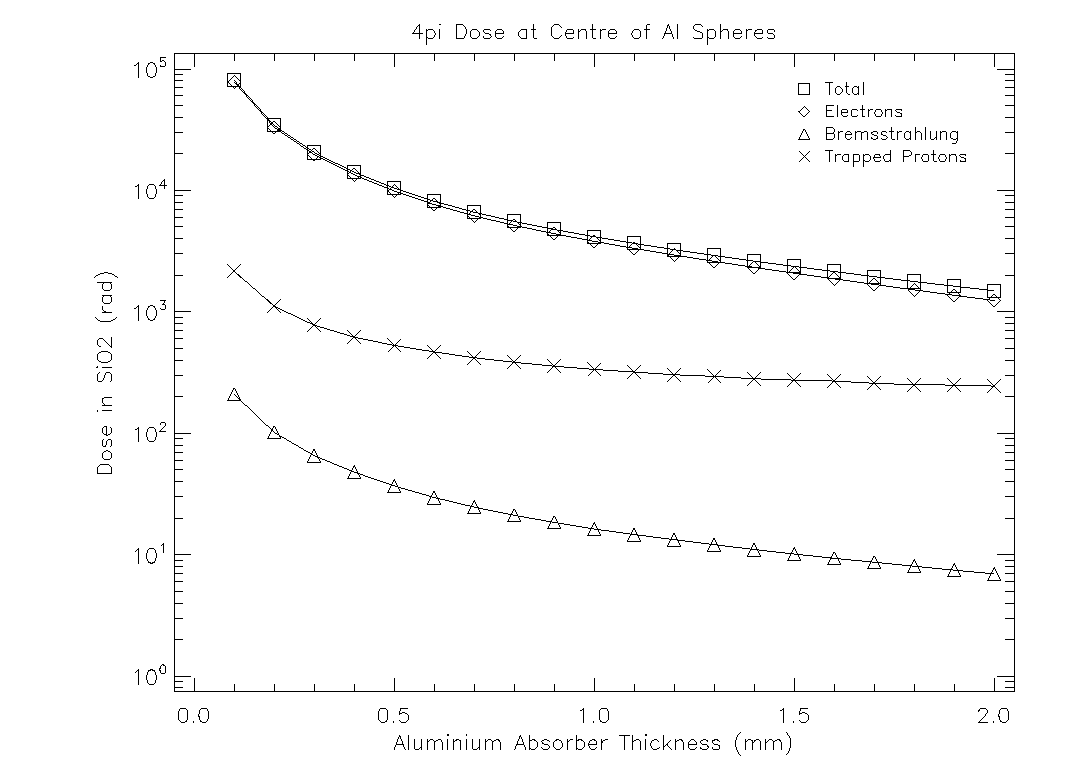
\includegraphics[width=0.58\paperwidth]{img/04/dose.eps}
            \caption{TID vs shielding during one year mission on \SI{575}{\kilo\meter} orbit}
            \label{TIDvsSheilding}
        \end{figure}

        The shielding of PW-Sat2 is about \SI{0.5}{\milli\meter} thick (aluminum sides as well as aluminum substrate for solar cells - \ref{PW-Sat_render_01}). Therefore, predicted dose during the primary mission is \SI{1}{\kilo\rad} and over the full, one year mission, is about \SI{10}{\kilo\rad}.

\section{Sensor requirements}
    Summing PW-Sat2 mission analysis, high-level sensor requirements were estimated, summarized in the table \ref{sensor_requirements_table}.

    \begin{table}[H]
        \caption{Sensor requirements}
        \label{sensor_requirements_table}
        \begin{center}
            \begin{tabular}{r|l}
                \textbf{Requirement} & \textbf{Value} \\ \hline
                Range & \SI{10}{\kilo\rad} \\
                Resolution & \SI{10}{\rad} \\
                Total accuracy & \SI{\pm 100}{\rad}
            \end{tabular}
        \end{center}
    \end{table}

\section{Applicable standards}
    The sensor should comply to ECSS \cite{ECSS_URL} standards. They are required by the launch provider and describe good practice during space product development.

    ESCIES \cite{ESCIES_URL} provides valuable knowledge about component qualification, testing and verification.

\section{Electrical requirements}
    The sensor will be placed on-board PW-Sat2. Therefore it should comply to its standards - power supplies, communication interfaces etc.

    \subsection{Electronics stack}
        Modules on PW-Sat2 are connected in the PC-104 stack structure as shown in the figure \ref{PW-Sat2_stack}. Is is placed inside the satellite housing and consists of (from the top):
        \begin{itemize}
            \item \textbf{Payload module (PLD)} - where the sensor will be located,
            \item On-Board Computer (OBC) - main data processing unit,
            \item Attitude Determination and Control Subsystem (ADCS) - controls attitude (detumbling and sunpointing),
            \item Electrical Power System (EPS) - charges and discharges batteries, provides safety mechanisms,
            \item Battery module (ACC) - main energy storage,
            \item Communication transceiver (COMM) - VHF \& UHF full duplex transceiver,
            \item Antennae module (ANT) - antennae for uplink and downlink.
        \end{itemize}

        \begin{figure}[H]
            \centering
            \includegraphics[width=0.5\paperwidth]{img/04/PW-Sat2-stack.png}
            \caption{PW-Sat2 electronics stack}
            \label{PW-Sat2_stack}
        \end{figure}

    \subsection{PC-104 connector}
        PLD board is connected to OBC with PC-104 connector. This connector provides data and power connections to the satellite bus.

        The connector consists of:
        \begin{itemize}
            \item $I^2C$ bus, connected directly to MCU on OBC,
            \item interrupt line on which the sensor can notify OBC about command completion,
            \item SENS \SI{5}{\volt} line, powered only when sensor is commanded to be enabled.
        \end{itemize}

    \subsection{Power rail}
        As mentioned earlier, the power for the sensor is +\SI{5}{\volt}, activated whenever the sensor is to be accessed by OBC.

        The power line is controlled and protected by a Latchup-Current Limiter FPF2701MX placed on the EPS board. Therefore, additional latchup protection in not necessary in this design. However, this sensor will not be the only one on the PLD board and should have its own power switch. The PLD board is enabled and disabled by EPS on the OBC command and the sensor should be enabled only during TID readout. Having this in mind forces the design to be immune to immediate shutdowns and dose have to be accumulated off-line.

    \subsection{Power consumption}
        During irradiation sensor should be completely turned off. It decreases possibility of radiation damage and increases overall system reliability.

        During readout the required power should be less than \SI{1}{W}.

    \subsection{Data interface}
        The sensor is connected to the OBC via the $I^2C$ interface. On this bus, OBC is the master, while the sensor is one of the slaves. The PLD board can be disabled and can therefore provide isolation of the $I^2C$ bus when it is powered off.

    \subsection{Radiation immunity}
        The design should itself be immune to radiation. For PW-Sat2, a threshold of \SI{10}{\kilo\rad} was chosen for all COTS components. Semiconductors should have radiation tests as described in \cite{ESCIES_TID_test_method}.

    \subsection{Electromagnetic compatibility}
        EMC requirements are described in \cite{ECSS_E_ST_20_07C}. This standard was tailored to PW-Sat2 because the power rail is \SI{+5}{\volt}, rather than the (\SI{+28}{\volt}) featured on bigger spacecraft.

        \begin{itemize}
            \item Conducted susceptibility is shown in the figure \ref{EMC_conducted_susceptibility} . It was created by down-scaling figure A-4 from \cite{ECSS_E_ST_20_07C} by factor of $\SI{28}{\volt}/\SI{5}{\volt} = 5.6$. The EMC limit on the power line is defined as a constant \SI{175}{\milli\volt} from \SI{30}{\hertz} to \SI{100}{\kilo\hertz}. The sensor should be able to filter this ripple to produce stable power for analog devices. In addition, it should be taken into account that output DC-DC converters on EPS run at \SI{500}{\kilo\hertz}.

            \begin{figure}[H]
                \centering
                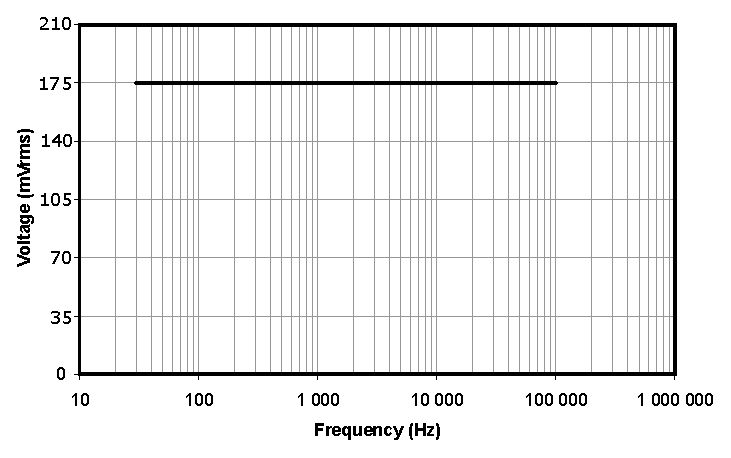
\includegraphics[width=0.5\paperwidth]{img/04/EMC_conducted_susceptibility.eps}
                \caption{Conducted susceptibility limit, frequency domain. Source: \cite{ECSS_E_ST_20_07C}}
                \label{EMC_conducted_susceptibility}
            \end{figure}


            \item Conducted emission is defined in the figure \ref{EMC_conducted_emission}.

            \begin{figure}[H]
                \centering
                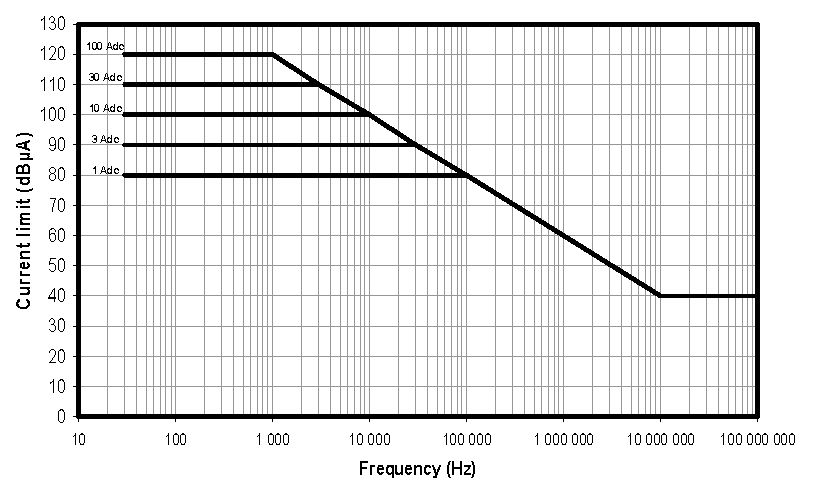
\includegraphics[width=0.5\paperwidth]{img/04/EMC_conducted_emission.eps}
                \caption{Conducted susceptibility limit, frequency domain. Source: \cite{ECSS_E_ST_20_07C}}
                \label{EMC_conducted_emission}
            \end{figure}


            \item Radiated susceptibility.
                On board PW-Sat2 is a communication module transmitting \SI{0.5}{\watt} of power at \SI{435.02}{\mega\hertz}. It is planned that during readout, the radio transmitter will be disabled, but proper tests should be conducted to check for possible errors and faults.

                PLD board is placed near OBC - so radiated emissions from digital lines can potentially couple to sensor elements causing noise and errors. Proper tests will be conducted and if necessary shielding will be implemented.

            \item Radiated emission.
                The sensor is not predicted to emit any kind of radio waves. In case of any detected anomalies, further design decisions would have to be made.

        \end{itemize}


    \subsection{Inrush current}
        Inrush current has to be limited to maximum power consumption to not trigger LCL on EPS (\SI{0.5}{\ampere}).

    \subsection{Reliability of components}
        This sensor is not a critical part of the satellite. Nonetheless, reliable components should be used to ensure proper results.

        Every used component should have a failure rate of $0.1\si{\percent}$ or lower. This is essential in capacitors and other passive components.

\section{Mechanical requirements}
    In this chapter design constraints and mechanical requirements of Falcon9 are presented. Launcher requirements were taken from \cite{Falcon9_user_manual}.

    \subsection{PCB}
    \label{PCB_description}
        PCB of PLD board is standard 4-layer FR4 board with stack shown in the figure \ref{PLD_PCB_stack}. Its dimensions are shown in the figure \ref{PLD_PCB_size}. The sensor design must, of course, occupy only a small amount of space on the board. For the sensor footprint, the limits are \SI{3x3}{\centi\meter} double sided.

        \begin{figure}[H]
            \centering
            \includegraphics[width=0.7\paperwidth]{img/04/PLD_PCB_stack.png}
            \caption{PLD board PCB stack}
            \label{PLD_PCB_stack}
        \end{figure}

        \begin{figure}[H]
            \centering
            \includegraphics[width=0.7\paperwidth]{img/04/PC104_PLD_size.png}
            \caption{PC-104 size}
            \label{PLD_PCB_size}
        \end{figure}



    \subsection{Outgassing}
        Every component used should be able to work in vacuum. Outgassing of components should be known to conduct required vacuum tests before launch. Too great an outgassing coefficient can result in damage to the turbomolecular pump in the vacuum chamber.

    \subsection{Vibration}
        During the rocket launch, large vibrations occur on the payload, therefore the rocket payload should be immune to vibration. In the case of heavy electronic components, appropriate glue should be applied to prevent joint cracks.
        \begin{figure}[H]
            \centering
            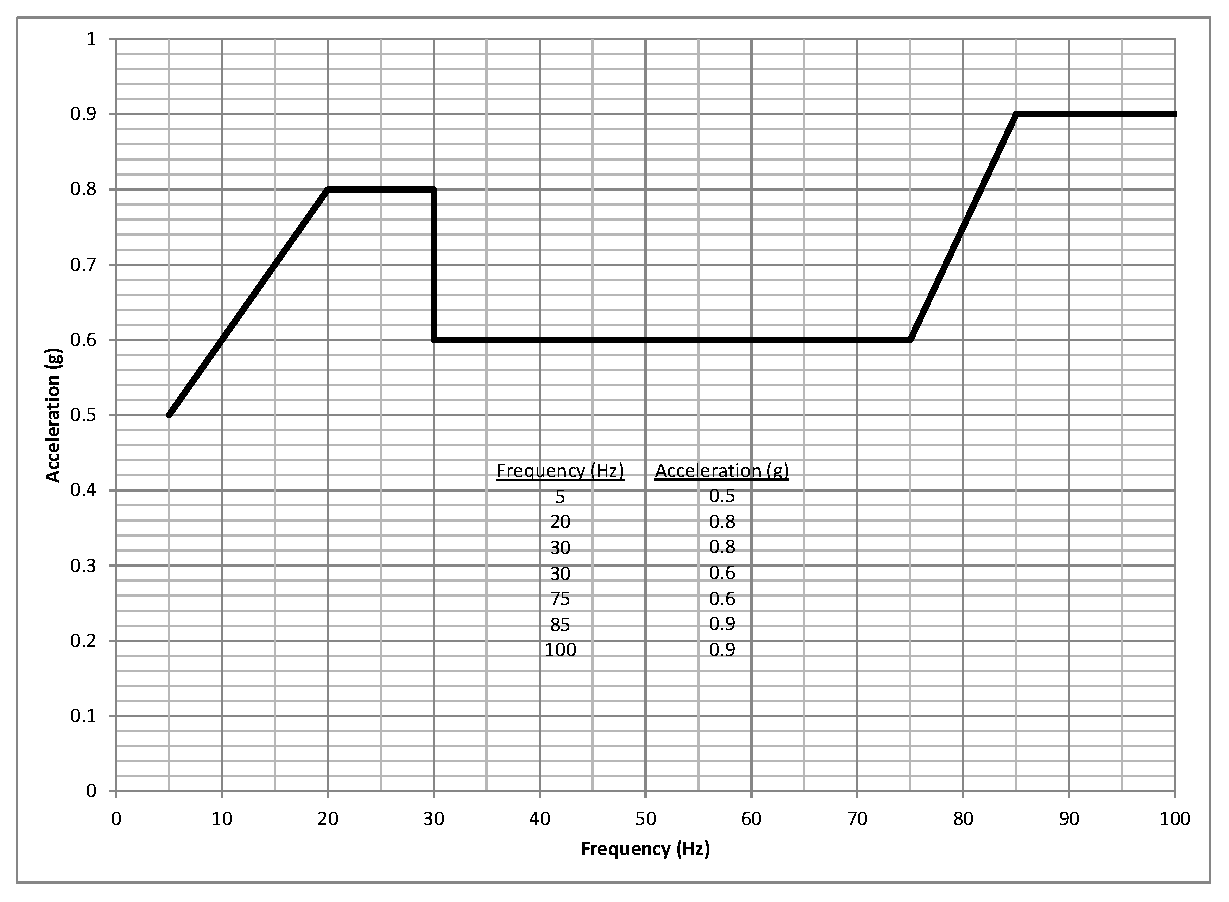
\includegraphics[width=0.5\paperwidth]{img/04/Falcon9_vibration.eps}
            \caption{Falcon9 maximum axial equivalent sine environment. Source: \cite{Falcon9_user_manual}}
            \label{Falcon9_vibration}
        \end{figure}


    \subsection{Operation temperature}
        The sensor should work in every operational case a satellite can be. Simulations were performed to find the boundaries of the  possible temperature range inside the satellite.    In \cite{PWSAT_TCS_CDR} results are presented.

        For the PLD board, the operation range is $\SI{0}{\degreeCelsius}$ to $\SI{60}{\degreeCelsius}$. If the measured temperature is outside this range, the sensor will not be enabled.


    \subsection{Thermal cycles}
        On the PW-Sat2 orbit, the sun illumination is changing every $\approx \SI{90}{\minute}$. Therefore a large number of thermal cycles are applied to the On-Board electronics, which can cause joint cracks as well as component failures. Proper soldering and component selection will be made, according to ECSS.

        As described in \cite{ECSS_Q_ST_70_04C} the sensor should pass thermal cycle tests: $100$ times from $- (100 \pm 5)$\si{\degreeCelsius} to $(100 \pm 5)$\si{\degreeCelsius} in a vacuum environment. This will be tested on Qualification Model.

% Design requirements
% - Sensor requirements
% -- Required sensitivity
% -- Required accuracy
% - Applicable standards
% - PW-Sat Mission
% -- Main purpose
% -- Orbit \& lifetime
% -- Radiation analysis
% - Electrical requirements
% -- Electronics stack
% -- Power
% -- Data interface
% -- Radiation immunity
% -- Reliability of components
% - Mechanical requirements
% -- PCB stack \& PCB restrictions
% -- Space available
% -- Vibration
% -- Operation temperature
% -- Thermal cycles

\chapter{Sensor design}
This chapter will cover sensor element selection, according to requirements presented previously.

Most space missions have on-board TID sensor - based od RadFET. RadFET is special type of modified p-MOSFET transistor, with well known dose dependence. In research work many COTS elements were checked for their characteristics, and they are now considered as a RadFET equivalent.

\section{RadFETs}
    Commercial solutions are based on modified MOS structure (with thicker gate region). Example silicon structure is show in figure \ref{Tyndall_radfet_silicon}. Different companies produce their own RadFET devices, by designing different structure, fitted to particular requirements. Found companies produce RadFET sensor alone, leaving readout circuit design for customer. Physical phenomena for RadFET sensors is described in section \ref{Physical_phenomena_background}.

    \begin{figure}[H]
        \centering
        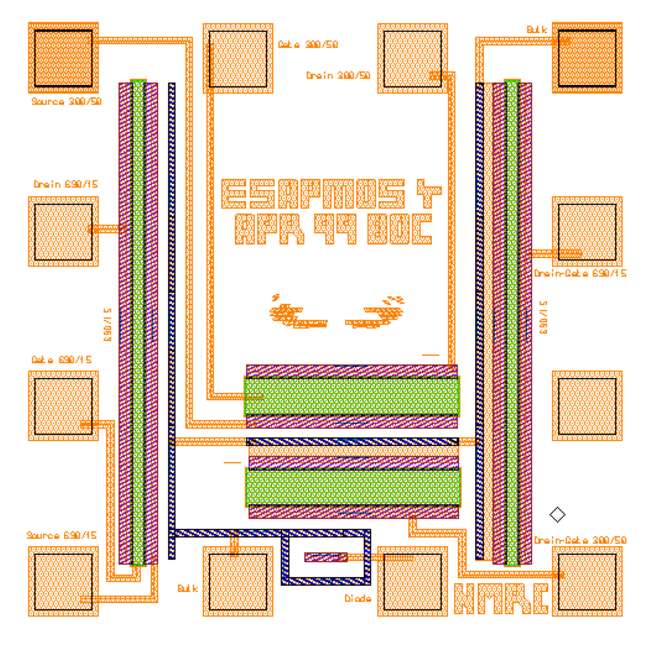
\includegraphics[width=0.5\paperwidth]{img/radfet-silicon.eps}
        \caption{4x RadFET silicon structure by Tyndall. Source: \cite{Tyndall_Radfet}}
        \label{Tyndall_radfet_silicon}
    \end{figure}


    Available products on market:

    \subsection{REM Oxford}
        REM Oxford \cite{RADFET_COM_URL}. This company produces RadFET type RFT300-CC10G1, its datasheet can be found on \cite{RFT300_CC10G1}. Structure is mounted on small carrier, as shown on figure \ref{REM_radfet_drawing}.

        \begin{figure}[H]
            \centering
            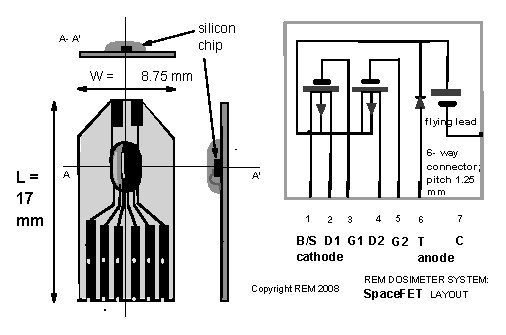
\includegraphics[width=0.5\paperwidth]{img/remOxfordDrawing.eps}
            \caption{RadFET made by REM Oxford. Source: \cite{RFT300_CC10G1}}
            \label{REM_radfet_drawing}
        \end{figure}

        This sensor consists of two PMOS transistors with modified gate structure.

        Key features:
        \begin{itemize}
            \item gate thickness \SI{200}{\nano\meter}, \SI{250}{\nano\meter} or \SI{300}{\nano\meter},
            \item sensitivity $\SI{1.5}{\milli\volt/\centi\gray} = \SI{1.5}{\milli\volt/\rad}$. Sensitivity chart is shown on figure \ref{REM_radfet_sensitivity}. At required sensitivity (\SI{1}{kRad}) threshold voltage shifts by $>\SI{100}{\milli\volt}$, depending on configuration,
            \item fading of shift is shown on figure \ref{REM_radfet_fading} - it is negligible on required mission duration ($<~\SI{3}{\percent}$),
            \item manufacturer suggests readout current in range $10-\SI{500}{\micro\ampere}$,
            \item sensor includes temperature readout from on-die diode
        \end{itemize}

        Price for one RadFET sensor begins from 800~\$.

        \begin{figure}[H]
            \centering
            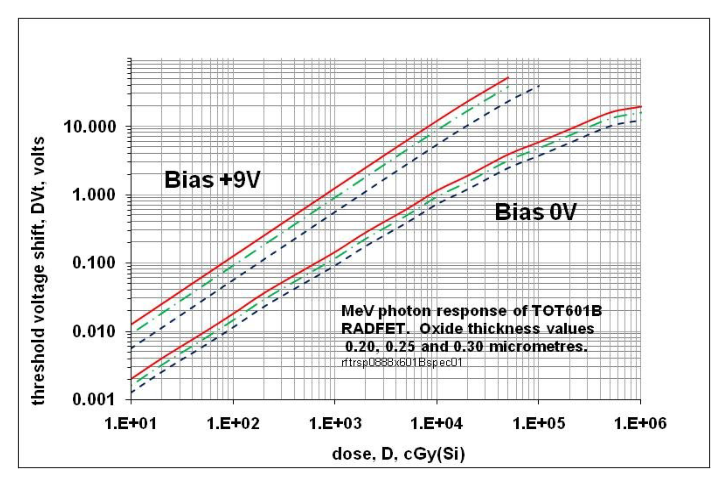
\includegraphics[width=0.6\paperwidth]{img/remSensitivity.eps}
            \caption{REM Oxford RadFET sensitivity. Source: \cite{RFT300_CC10G1}}
            \label{REM_radfet_sensitivity}
        \end{figure}

        \begin{figure}[H]
            \centering
            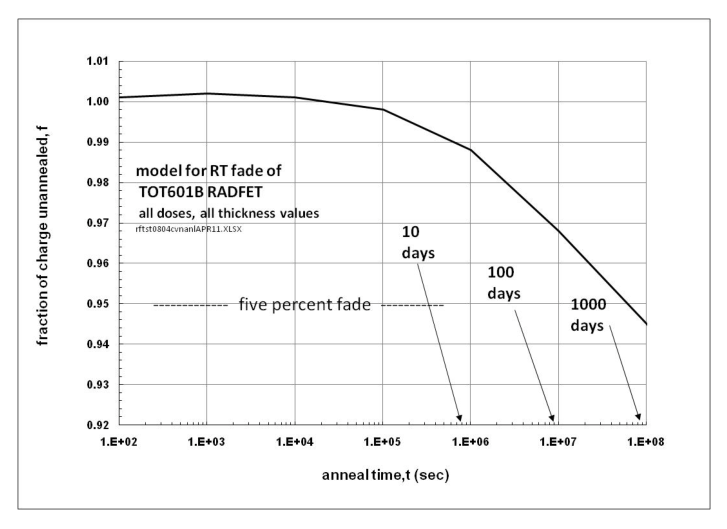
\includegraphics[width=0.6\paperwidth]{img/remOxfordFading.eps}
            \caption{REM Oxford RadFET fading. Source: \cite{RFT300_CC10G1}}
            \label{REM_radfet_fading}
        \end{figure}


    \subsection{Tyndall}
        Tyndall Works manufactures RadFET components in different packaging options \cite{TYNDALL_URL}. They provide calibration data for each type of sensor, as their response is very non-linear. Graph showing sensitivity of TY1002 is shown on figure \ref{Tyndall_TY1002_sensitivity}. Tyndall provide 4 different options, their comparison is done in table \ref{Tyndall_comparison}. Tyndall recommends grounding RadFET terminals during irradiation.

        \begin{figure}[H]
            \centering
            \includegraphics[width=0.6\paperwidth]{img/Tyndall_TY1002_sensitivity.png}
            \caption{Tyndall TY1002 sensitivity. Source: \cite{TYNDALL_URL}}
            \label{Tyndall_TY1002_sensitivity}
        \end{figure}

        \begin{table}[H]
        \begin{tabular}{| L{3.5cm} | C{2.5cm} | C{2.5cm} | C{2.5cm} | C{2.5cm} |}
            \hline
            Type: & TY1001 & TY1002 & TY1003 & TY1004 \\ \hline

            Image: &
            \includegraphics[width=0.12\paperwidth]{img/TY1001.png} &
            \includegraphics[width=0.12\paperwidth]{img/TY1002.png} &
            \includegraphics[width=0.12\paperwidth]{img/TY1003.png} &
            \includegraphics[width=0.12\paperwidth]{img/TY1004.png} \\ \hline

            Package: & 14-pin ceramic DILpin ceramic DIpin ceramic DI & SOT-23 & SOT23-6 & 8-pin ceramic DIL \\ \hline

            \# of transistors: & 4 & 1 & 2 & 2 \\  \hline
            W/L : & 300/50 \& 690/15 & \multicolumn{3}{c|}{300/50}  \\  \hline
            Oxide thickness: & - & - & \multicolumn{2}{c|}{\SI{400}{\nano\meter}} \\  \hline

            Maximum dose: & \multicolumn{4}{c|}{\SI{100}{\kilo\rad}} \\  \hline
            Minimal detectable dose: & \multicolumn{4}{c|}{\SI{1}{\rad}} \\  \hline

            Recommended readout current: & \multicolumn{2}{c|}{\SI{12.5}{\micro\ampere}} & \multicolumn{2}{c|}{\SI{10}{\micro\ampere}} \\ \hline

            Temperature readout: & diode & none & diode & diode \\ \hline
        \end{tabular}
        \caption{Tyndall RadFET comparison}
        \label{Tyndall_comparison}
        \end{table}


\section{MOSFET as RadFET}
    COTS transistors parameters also depends on total dose - but in less predictable way. But this solution is much cheaper, and after self-made calibration can be considered as flight solution. According to papers, many transistors were already measured by different scientific teams. For this thesis couple of them were selected for comparison.

    P-MOSFET can have different characteristics (lower slope, higher drift and fading) than commercial RadFETs, but considering cost and space it is unfeasible for implementing RadFET-based sensor on PW-Sat2.



\section{Chosen MOSFET: CD4007}

\section{Conceptual Block diagram}

    Conceptual block diagram is presented on figure TODO. It consists of mosfet, current source, analog to digital converter and die temperature measurement. Description is presented below.

    \subsection{Thresold voltage}
        According to theory, to measure TID accumulated threshold voltage in transistor have to be measured. The simplest solution is to use current source connected to MOSFET in diode connection. Measured voltage is not true threshold voltage which literature refers to, but this is enough for TID measurements, because absolute value of $V_{th}$ does not matter - only it's shift. From now, this thesis will refer to $V_{th}$ defined as $V_{GS}$ at a given drain current.

        During irradiation current source should be disabled - as well as the whole sensor. This will lead to no power consumption during irradiation, enabling device only for readout.

    \subsection{Die temperature}
        Because measured threshold voltage strongly depends on die temperature this effect have to be compensated. According to papers, predicted dependence $V_{th}(TID)$ is about $TODO$ and temperature shift is \SI{-2}{\milli\volt/\kelvin}. Therefore die temperature have to be measured very accurately, and individual MOSFET will have to be calibrated prior to launch.

        Couple of options were considered during this thesis:
        \begin{itemize}
            \item discrete PT-1000 sensor glued to MOSFET - this was rejected because of large heat resistance,
            \item ESD diode measurement in CD4007 - readout circuit for this solution is rather complicated, therefore it was rejected too,
            \item body diode in N-MOSFET in CD4007 package - this is chosen solution
        \end{itemize}

        Temperature dependence of body diode in N-MOSFET can be calibrated on ground. N-MOSFETs are placed very close to P-MOSFETs in CD4007, therefore temperature measurement will be very accurate.

        Is is planned to use the same current source for both threshold voltage and temperature measurements - and to multiplex it. This will lead to very simple readout circuit, having in mind space restrictions.

\section{Characteristic curves (MG)}
\section{Operating point selection}

% Sensor design
% - Commercial RadFETs
% - Review of commercially available RadFETs
% - Selected MOSFET - CD4007
% - Conceptual Block diagram
% - Characteristic curves (MG)
% - Operating point selection

\chapter{Engineering model}
This chapter will describe engineering model developed during this thesis.

This model should be as close to flight model as possible - but it could be e.g. on separate board, which is this case.

This model was developed as flight-ready version for sensor calibration \& tests along with developing \& testing flight software.

\section{Background - calibration stand}
    During development of the system previous model was developed to test and calibrate MOSFET transistors to use as a radiation dosimeters. Calibration stand was developed by M. Gumiela in his engineering thesis \cite{MGThesis}. The basic goal was to develop measurement device which can be used to determine final operational point, calibrate radiation response and to perform temperature calibration of flight sensor.

    TODO: opis stanowiska


\section{Block diagram}
    Block diagram of proposed system based on CD4007 is presented on figure TODO.

    It was designed having in mind miniaturization of sensor - to fit on PW-Sat2 PLD board. Because CD4007 has 3 complementary MOS pairs it was proposed to use all of them - to improve fidelity of the measurements. One n-MOS is used as a temperature sensor.

    Current source and ADC are multiplexed between 4 channels - 3x p-MOS and 1x n-MOS. This reduces board space and sensor accuracy (1 current source/ADC can be more sophisticated).

\section{Low-level requirements}
    Using design requirements \ref{Design_requirements} and characteristic curves from \ref{Characteristic_curves} low-level specifications were assumed:
    \begin{itemize}
        \item operating temperature range: $0 \div 60 \si{\degreeCelsius}$,
        \item current source value: $\SI{100}{\micro\ampere} \pm \SI{10}{\nano\ampere}$,
        \item ADC resolution: $TODO$,
        \item ADC accuracy: $TODO$,
        \item Noise floor on ADC: $TODO$
    \end{itemize}


\section{Analog front-end}
    In this section decision and schematic diagrams of building blocks are presented.

    \subsection{SPICE models}
        Design should be validated by simulation. To make this possible, model of every device should be accessible.

        For CD4007 model RIT4007P7 from Rochester Institute of Technology \cite{RIT_FULLER} was used.

    \subsection{Linear regulator}
        Important part of design - power supply for analog circuitry. Because $+\SI{5}{V}$ rail from EPS is an output from DC-DC converter (which runs on \SI{500}{\kilo\hertz}) the analog supply voltage have to be very well regulated and filtered. Because line from satellite bus is \SI{5}{\volt} and to run current source there is a need for as high voltage as possible LDO output voltage was selected to be \SI{4.5}{\volt}.

        As an Low Dropout Voltage LT3042 was selected. It is ultralow Noise, ultrahigh PSRR RF linear regulator by Linear Technology. Key specs:
        \begin{itemize}
            \item ultralow noise \SI{0.8}{\micro\volt RMS} (\SI{10}{\hertz} to \SI{100}{\kilo\hertz}),
            \item output current \SI{200}{\milli\ampere}
            \item input range \SI{1.8}{\volt} to \SI{20}{\volt}, output range \SI{0}{\volt} to \SI{15}{\volt}
            \item ultrahigh PSRR \SI{79}{\decibel} at \SI{500}{\kilo\hertz}
        \end{itemize}

    \subsection{Current source}
        Current source have to be the most accurate part of the design, because measured voltage depends in square of its variation. It was assumed that $\SI{50}{\nano\ampere}$ current stability across temperature and aging range will be sufficient.

        Main concept of current source is based on Burr-Brown application note \cite{Make_a_precision_current_source_or_sink}. Idea schematic is shown on figure \ref{current_source_schematic}.

        \begin{figure}[H]
            \centering
            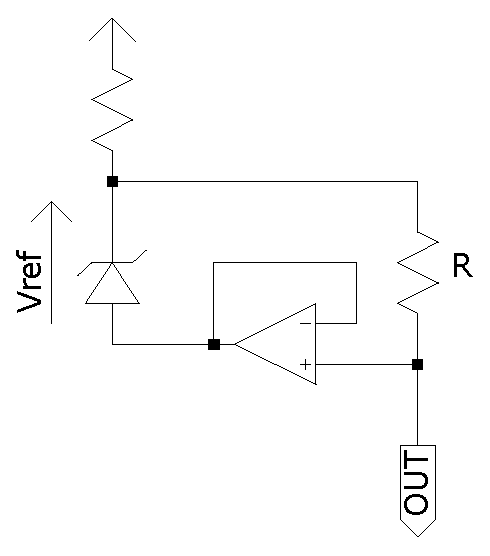
\includegraphics[width=0.3\paperwidth]{img/06/current_source_schematic.eps}
            \caption{Threshold voltage readout block diagram}
            \label{current_source_schematic}
        \end{figure}

        Output current is set by shunt voltage reference and resistor $R$, it is given by equation:
        $$I_{OUT} = V_{ref}/R$$

        Therefore, stability of output current depends on reference voltage and resistor accuracy.

        \bigskip \textbf{Shunt reference}

        After irradiation MOSFET $V_{DS}$ is planned to be about \SI{2.5}{\volt}, so reference voltage have to have voltage less than \SI{2}{\volt}.

        Linear Technology LT1634-1.25 shunt voltage reference was chosen. It is one of the best shunt references from LT. Basic specification:
        \begin{itemize}
            \item \SI{0.05}{\percent} initial accuracy,
            \item \SI{10}{ppm/\degreeCelsius} maximum temperature drift,
            \item $< \SI{1}{\ohm}$ dynamic resistance
        \end{itemize}

        Shunt resistance was chosen to make a current flowing through reference about $10-\SI{20}{\micro\ampere}$ - value of \SI{5}{\kilo\ohm}.

        \bigskip \textbf{Series resistor}

        Value of this resistor reflects required current flowing through MOSFET. Nominal value selected was $TODO$.

        Critical in this resistor is stability across temperature, it directly reflects changes in current. For achieving requirements \SI{10}{\kilo\ohm} / \SI{5}{ppm} was chosen (APC0603T10K0Z).

        Manufacturer does not specify profile of the temperature coefficient - so both worst cases was simulated (\SI{-5}{ppm} and \SI{5}{ppm}).

        \bigskip \textbf{Operational amplifier}

        Operational amplifier in this circuit have very low bandwidth (noise limitation), low offset voltage (precision) and small footprint. LTC2054 was selected - key characteristics:
        \begin{itemize}
            \item \SI{3}{\micro\volt} offset voltage,
            \item common mode $\pm \SI{0.5}{\volt}$ input/output range,
            \item \SI{500}{\kilo\hertz} gain-bandwidth product,
            \item device in Military Plastic package (temperature range $-55 \div \SI{150}{\degreeCelsius}$)
        \end{itemize}

        \bigskip \textbf{Simulation}

        Full behavioral simulation was performed in LTSpice. MOSFET was replaced by resistance emulating its static resistance ($\SI{2}{\volt}/\SI{125}{\micro\ampere} = \SI{16}{\kilo\ohm}$). Simulation view is shown on figure \ref{current_source_simulation}.

        \begin{figure}[H]
            \centering
            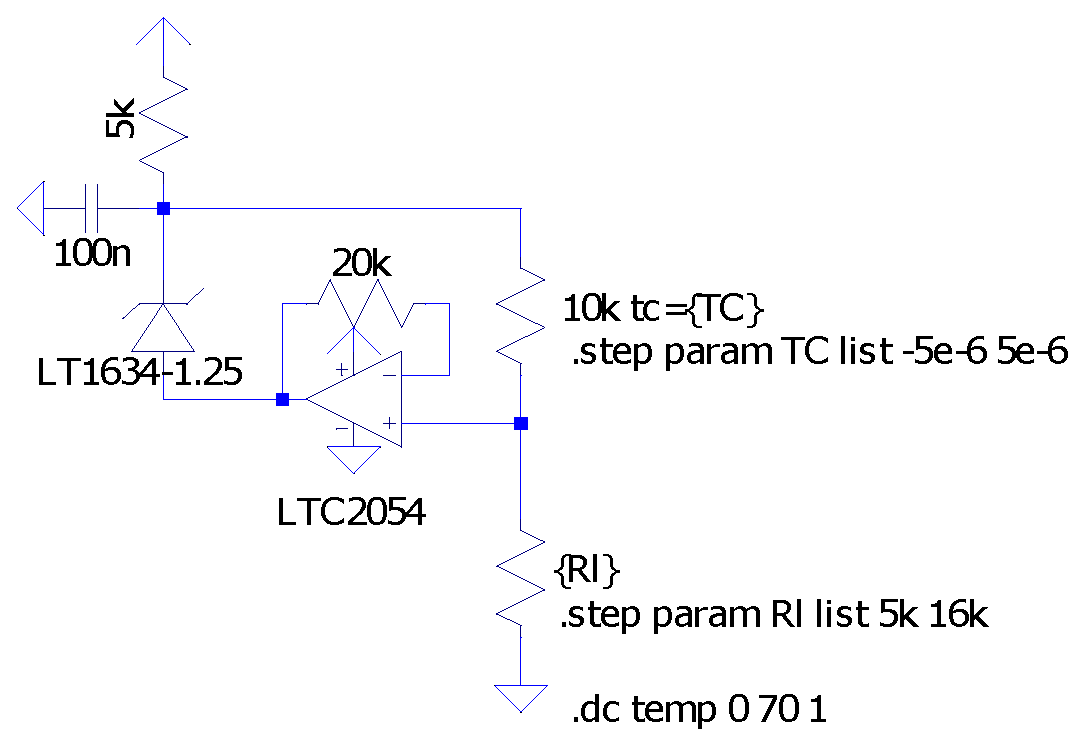
\includegraphics[width=0.5\paperwidth]{img/06/current_source.eps}
            \caption{Current source simulation}
            \label{current_source_simulation}
        \end{figure}

        Result (output current):

        \begin{figure}[H]
            \centering
            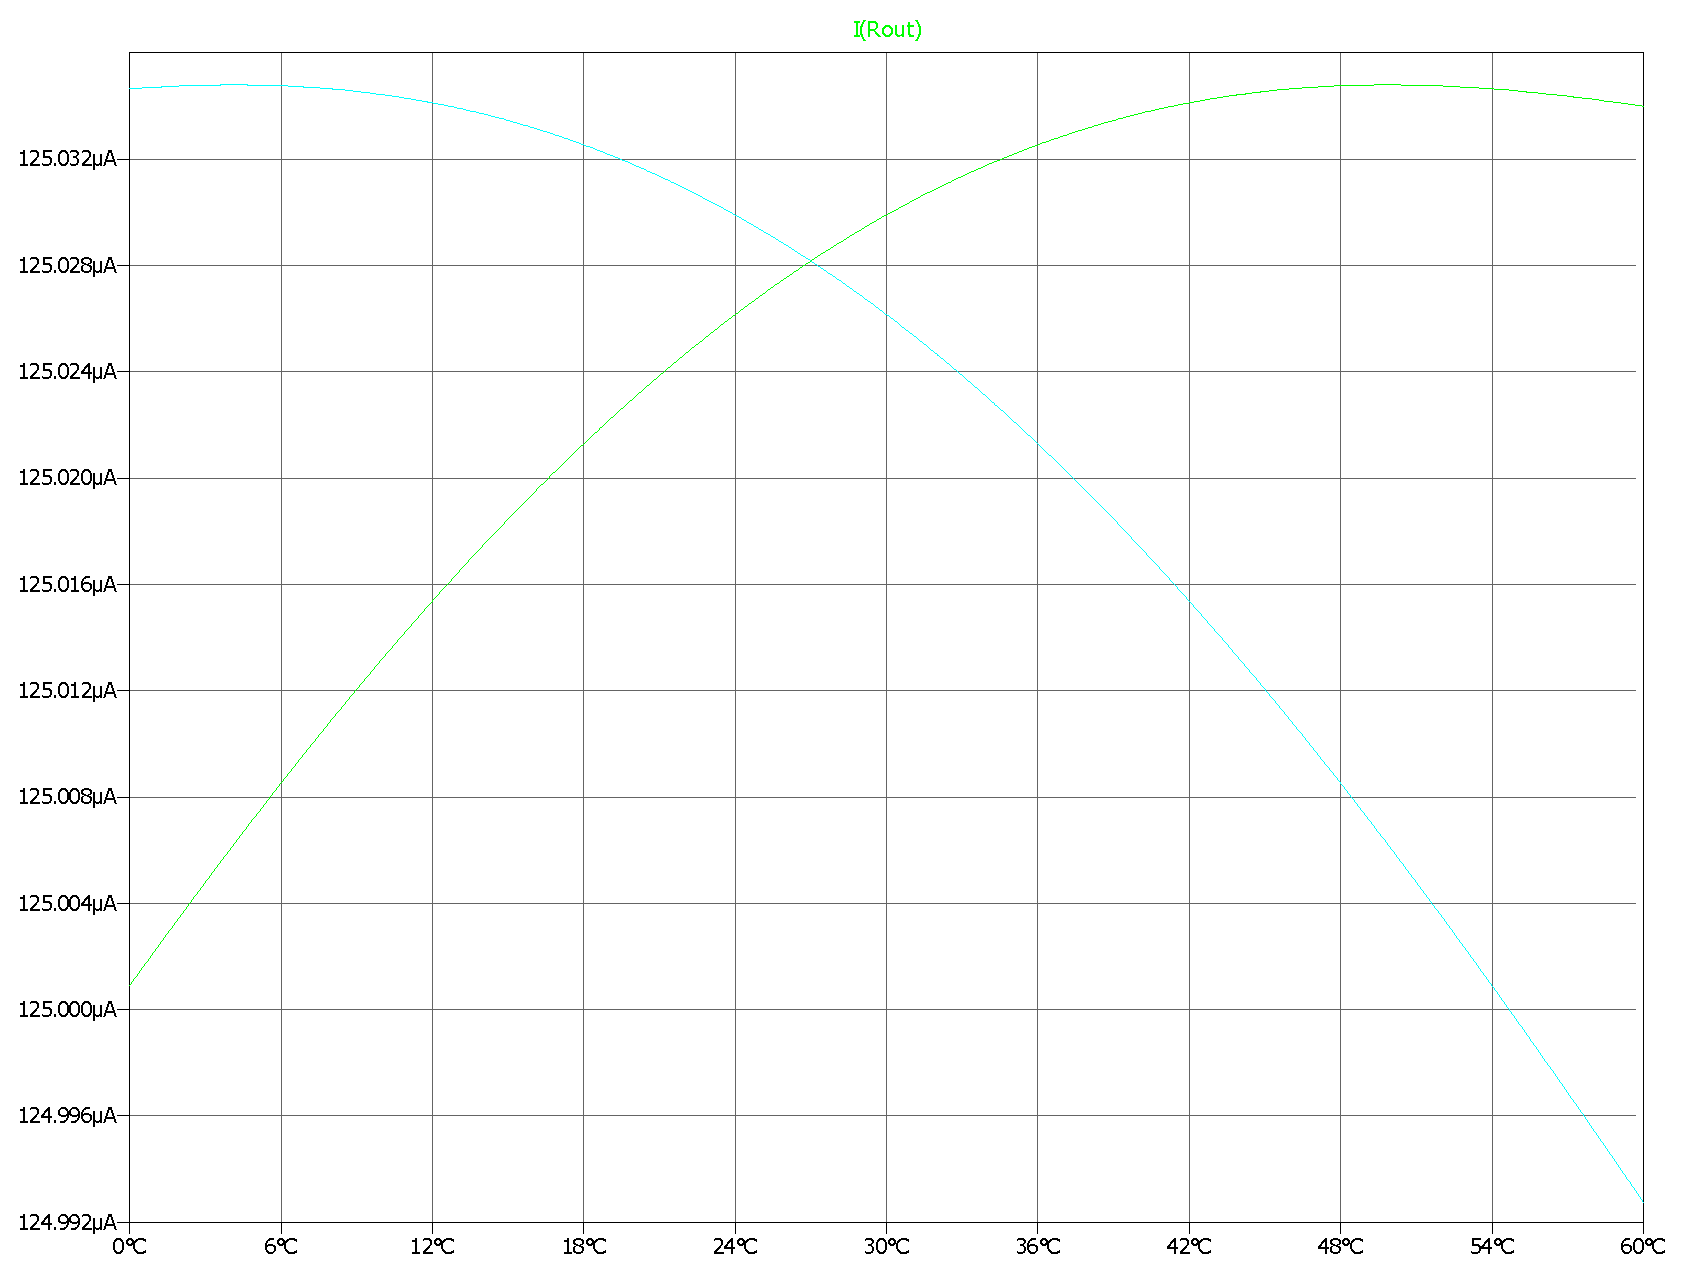
\includegraphics[width=0.8\paperwidth]{img/06/current_source_result.eps}
            \caption{Current source simulation result - output current}
            \label{current_source_simulation_result}
        \end{figure}

        In both cases current change across temperature range does not exceed \SI{40}{\nano\ampere}.

    \subsection{ADC}
        Analog to digital converter is responsible for reading $V_{DS}$ voltage across transistor. Due to very low changes high accuracy and resolution is required. Additionally, complex digital element like ADC should have radiation tests to prove its reliability. To achieve at least \SI{0.1}{\milli\volt} resolution ADC has to be at least \SI{16}{bits}.

        Due to constrain on system and reliability the AD7714 from Analog Devices was chosen. Radiation tests for this device can be found at TODO. Internal diagram can be found on figure \ref{AD7714}. Key specs:
        \begin{itemize}
            \item \SI{24}{bits},
            \item \SI{0.0015}{\percent} nonlinearity,
            \item programmable gain ($1 \div 128$),
            \item 3 fully differential or 5 pseudo-differential input channels
            \item \SI{3}{\volt} or \SI{5}{\volt} operation
            \item separated digital and analog supply and grounds,
            \item SPI interface
        \end{itemize}

        \begin{figure}[H]
            \centering
            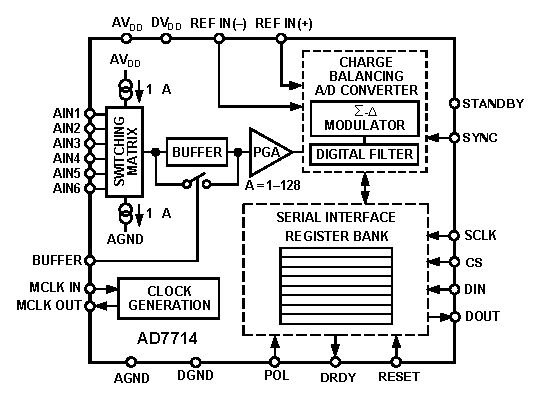
\includegraphics[width=0.5\paperwidth]{img/06/AD7714.eps}
            \caption{AD7714 internal block diagram. Source: TODO}
            \label{AD7714}
        \end{figure}

        This ADC is much too complex for this particular need, but it is the only one (apart from ADC128, but this is 12-bit) with radiation tests.

        AD7714 requires external crystal or clock oscillator in frequency range \SI{1}{\mega\hertz} to \SI{2.54}{\mega\hertz}. Crystal oscillators for these frequencies are large and susceptible for shocks and damages because of large, delicate internal structure (firure \ref{Opening_a_Quartz_Crystal_Can_Effects_Thereof}). \SI{1}{\mega\hertz} ceramic oscillator ISM95-3351AH was selected for operation (figure \ref{ISM95-3351AH-1.0000}).

        \begin{figure}[H]
            \centering
            \includegraphics[width=0.5\paperwidth]{img/06/crystal.png}
            \caption{Low frequency crystal oscillator internals. Source: \cite{        Opening_a_Quartz_Crystal_Can_Effects_Thereof}}
            \label{Opening_a_Quartz_Crystal_Can_Effects_Thereof}
        \end{figure}

        \begin{figure}[H]
            \centering
            \includegraphics[width=0.5\paperwidth]{img/06/ISM95.png}
            \caption{ISM95-3351AH-1.0000 ceramic oscillator package. Source: TODO}
            \label{ISM95-3351AH-1.0000}
        \end{figure}


    \subsection{Multiplexer}
        Because CD4007 have three p-MOS transistors it was planned to read every channel. Space constrains does not allow to have four current sources (for p-MOS and n-MOS), therefore current have to be multiplexed. Additionally, ADC have only three differential input, so it was proposed to multiplex it as well.

        As an analog multiplexer ADG709 was chosen. Its radiation tests can be found in TODO. It is double 1:4 mux, allowing simultaneous current and voltage multiplexing. Internal block diagram is shown on figure \ref{ADG709_block}

        \begin{figure}[H]
            \centering
            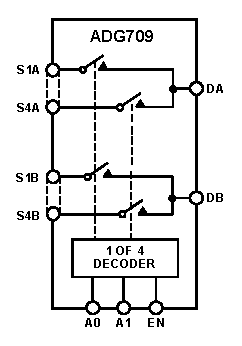
\includegraphics[width=0.3\paperwidth]{img/06/ADG709.eps}
            \caption{ADG709 internal block diagram. Source: TODO}
            \label{ADG709_block}
        \end{figure}

    \subsection{Differential filter}
        Internal sampling frequency of ADC (for GAIN = 1 and $f_{clk} = \SI{1}{\mega\hertz})$ is about \SI{15.6}{\kilo\hertz}. To eliminate aliasing and reduce readout noise low-pass differential filter should be implemented on ADC input.

        Simple one-pole RC filter was selected. Its schematic can be found on figure \ref{low_pass_filter}.

        \begin{figure}[H]
            \centering
            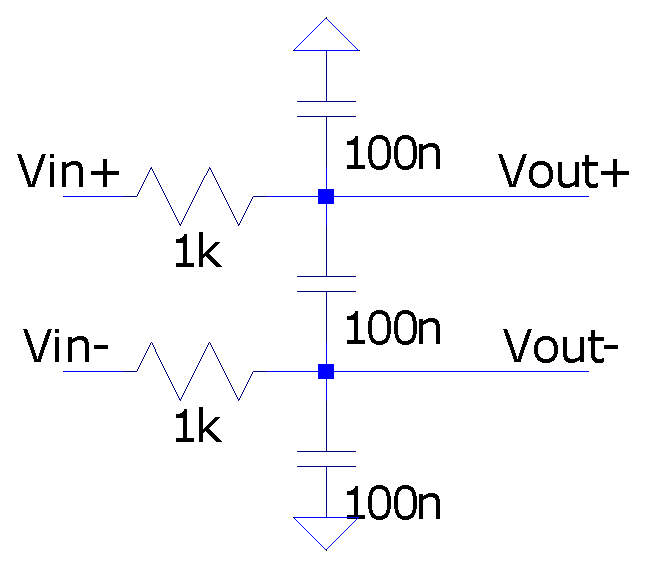
\includegraphics[width=0.3\paperwidth]{img/06/low_pass_filter.eps}
            \caption{Low pass filter schematic.}
            \label{low_pass_filter}
        \end{figure}

        Using AC analysis its frequency characteristic was obtained - figure \ref{low_pass_filter_output}. At half of sampling frequency attenuation is about \SI{22}{\decibel}.

        \begin{figure}[H]
            \centering
            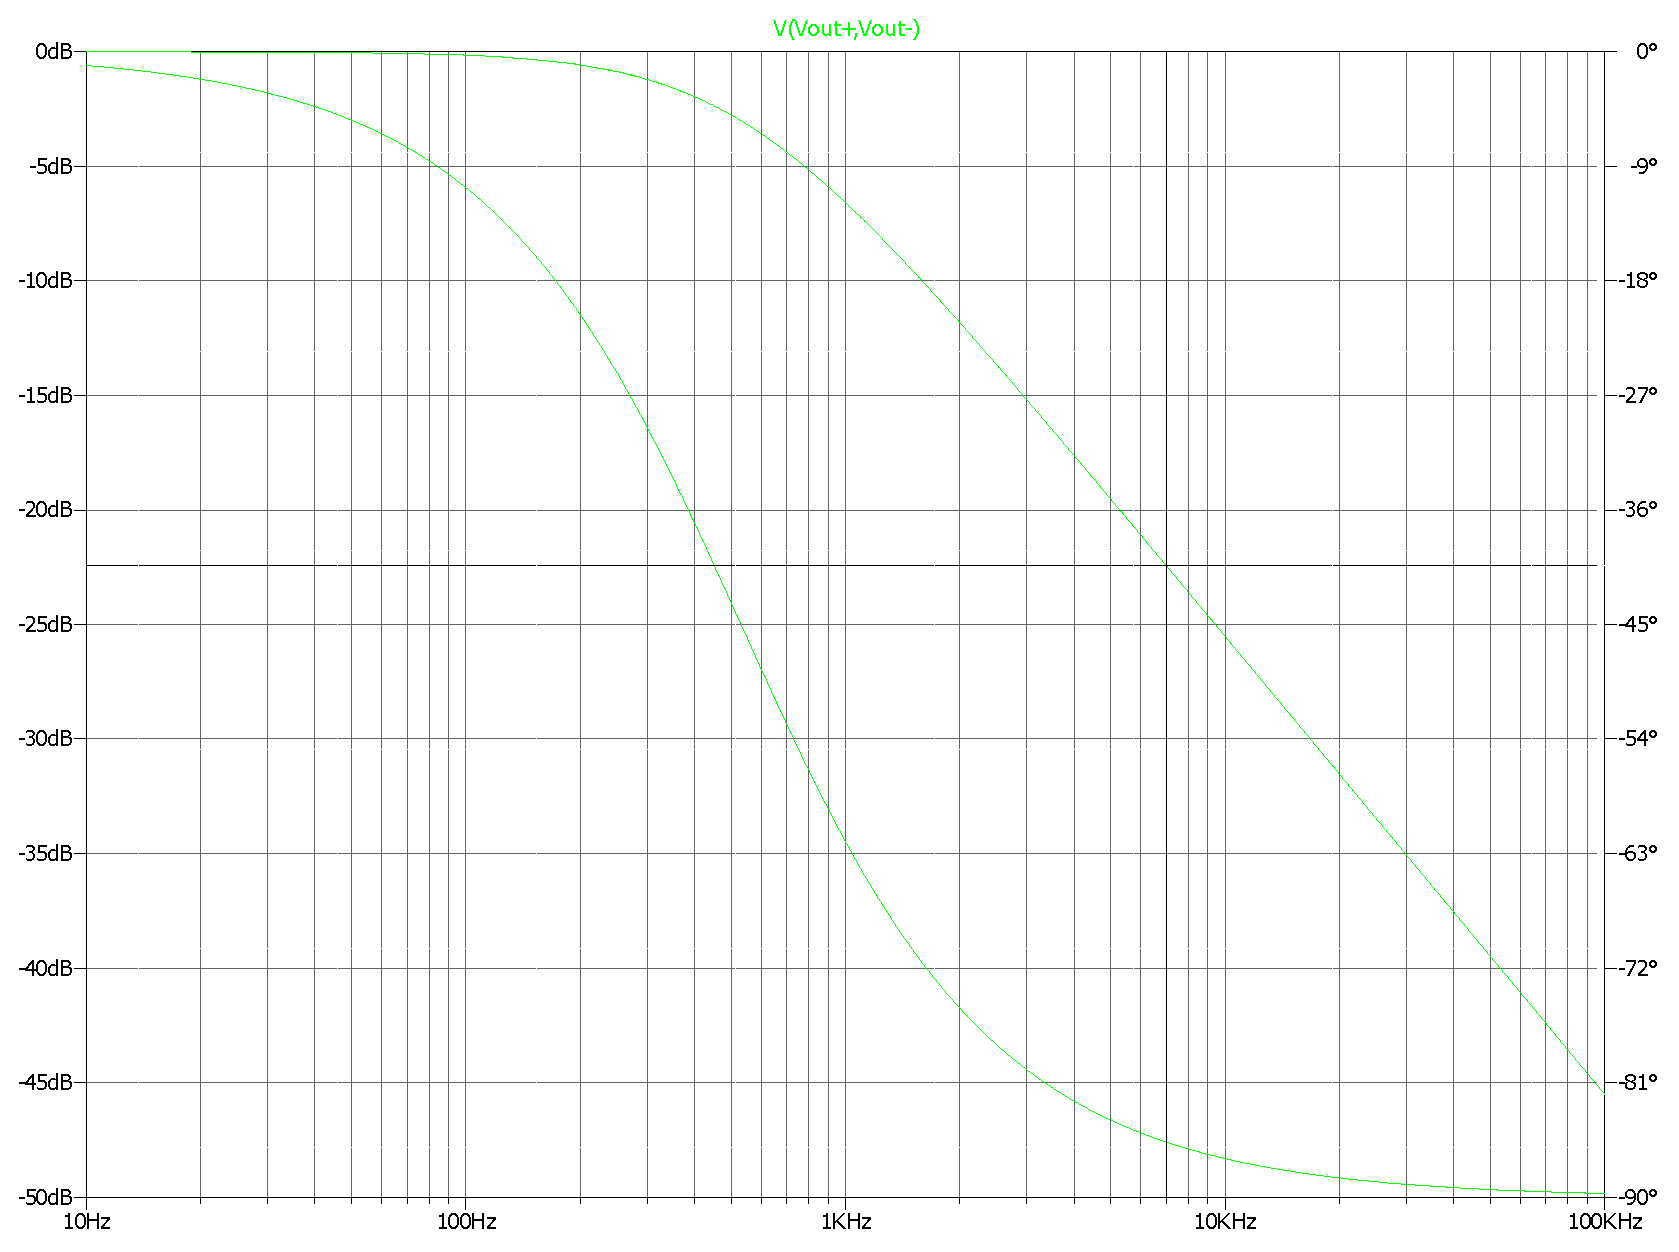
\includegraphics[width=0.7\paperwidth]{img/06/low_pass_filter_output.eps}
            \caption{Low pass filter frequency characteristics.}
            \label{low_pass_filter_output}
        \end{figure}

    \subsection{Shielding}
        Because of noise requirements and near proximity of \SI{0.5}{\watt} radio transmitter, EMI shielding was tested.

        Proper pads for EMI shielding were placed on PCB. Its size depends on PCB layout, after routing it was decided to use BMI-S-203 shield (figure \ref{BMI-S-203}). This shield should provide attenuation of about \SI{50}{\decibel} on transmitter frequency.

        \begin{figure}[H]
            \centering
            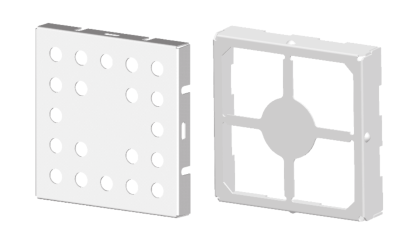
\includegraphics[width=0.7\paperwidth]{img/06/BMI-S-203.eps}
            \caption{BMI-S-203 shield. Source: TODO}
            \label{BMI-S-203}
        \end{figure}


\section{Digital}
    RadFET is mainly analog sensor. But, ADC, MUX and LDO has to be controlled from on-board microcontroller. On other hand, RadFET have to be accessible from OBC, to retrieve data and send them to ground.

    \subsection{Microcontroller}
        Main digital part of the design is microcontroller. It will be responsible for:
        \begin{itemize}
            \item controlling analog part of the sensor,
            \item calculating values and implement FDIR for incorrect values,
            \item communicating with OBC to send data and transfer them to ground station for further analysis.
        \end{itemize}

        Couple of options were considered, and the final choose was ATmega164PV-10AQ.

        AVR devices are known from their simplicity, reliability and very little bugs. In addition, radiation tests were performed for ATmega series (TODO).

        Features of this particular device:
        \begin{itemize}
            \item \SI{1.8}{\volt} - \SI{5.5}{\volt} supply voltage,
            \item \SI{4}{\mega\hertz} clock,
            \item TQFP-44 package,
            \item \SI{16}{\kilo B} program memory,
            \item \SI{1}{\kilo B} SRAM
        \end{itemize}

    \subsection{OBC interface}
        Interface to OBC is $I^2C$ bus. Because sensor can be turned off by cutting its voltage proper buffering had to be implemented. For this purpose $I^2C$ repeater PCA9517 was placed in the design. Its functional diagram can be seen on figure \ref{PCA9517}. From its datasheet: "The SDA and SCL pins are over voltage tolerant and are high-impedance when the PCA9517 is unpowered." (TODO). Thanks to it OBC can completely disable the sensor, by simply cutting it a power.

        \begin{figure}[H]
            \centering
            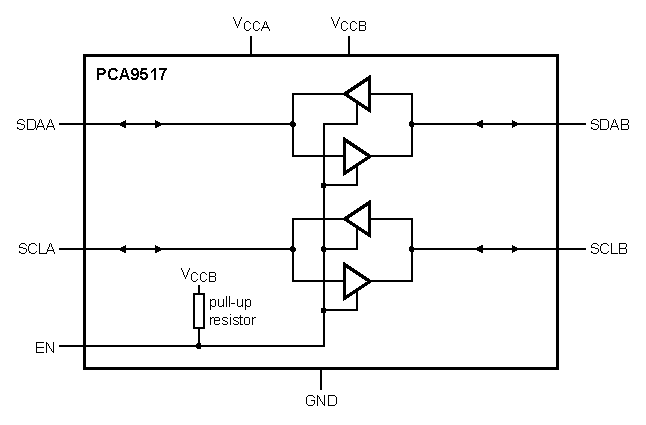
\includegraphics[width=0.7\paperwidth]{img/06/PCA9517.eps}
            \caption{PCA9517 internal block diagram. Source: TODO}
            \label{PCA9517}
        \end{figure}


\section{Final schematic}
    Top level schematic file can be seen on figure \ref{top_level_schematic}. Ports represents physical connectors - to satellite bus and debug socket.

    \begin{figure}[H]
        \centering
        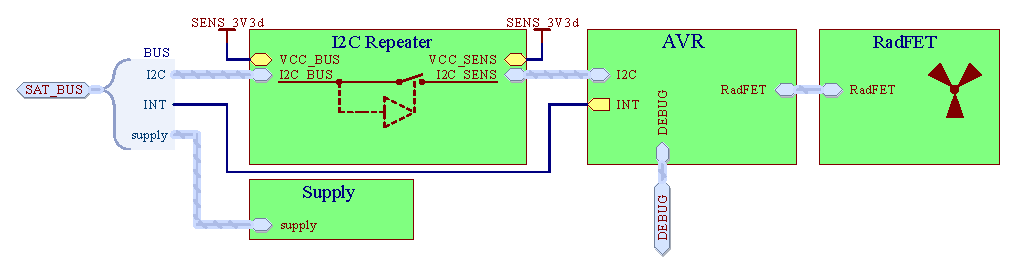
\includegraphics[width=0.8\paperwidth]{img/06/final_schematic_top.eps}
        \caption{Top level schematic}
        \label{top_level_schematic}
    \end{figure}

    "RadFET" consists analog part of the design. Its block diagram can be seen on figure \ref{analog_schematic}.

    \begin{figure}[H]
        \centering
        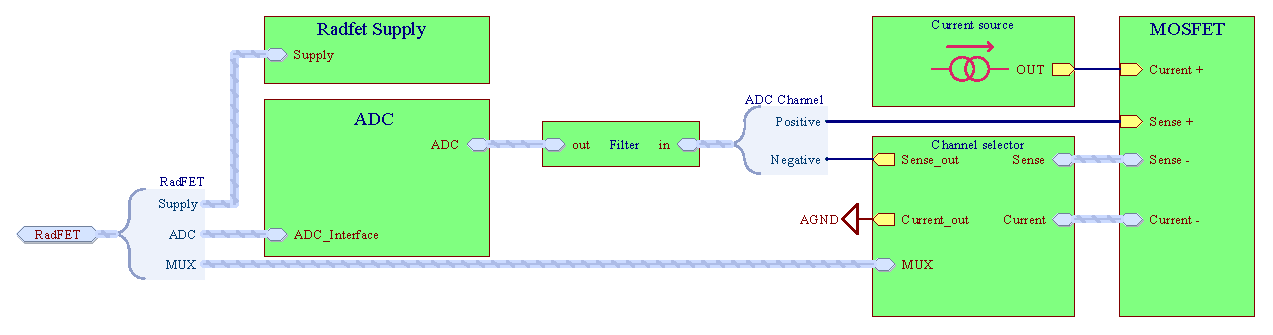
\includegraphics[width=0.8\paperwidth]{img/06/final_schematic_radfet.eps}
        \caption{Sensor final schematic - analog part}
        \label{analog_schematic}
    \end{figure}


\section{Software design}
    \subsection{AVR-HAL}
    \subsection{I2C-slave module}
    \subsection{Measurement algorithm}

\section{PCB}
    \subsection{PCB stack}
    \subsection{PCB layout}
    \subsection{3D model}
    \subsection{Manufacturing}

\section{Assembly}

\section{Finished sensor}

% Engineering model
% - Background - calibration stand
% - Block diagram
% - Low-level requirements
% - Analog front-end
% -- Current source
% -- ADC
% -- Multiplexer
% -- LDO
% -- Shielding
% - Digital
% -- Microcontroller
% -- OBC interface
% - Software design
% -- AVR-HAL
% -- I2C-slave module
% -- Measurement algorithm
% - PCB
% -- PCB stack
% -- PCB layout
% -- 3D model
% -- Manufacturing
% - Assembly
% - Finished sensor

\chapter{Sensor tests}

%\section{Digital}
%    \subsection{Interface tests}
%    \subsection{Software tests}

\section{Power}
    \subsection{LDO stabilisation}
        Voltage after LDO was measured in time, to calculate delay between power enable and measurement start. Time graph is shown on figure \ref{LDO_rise_time}. Delay was estimated to be around \SI{1}{\second}.

        \begin{figure}[H]
            \centering
            \includegraphics[width=0.8\paperwidth]{img/07/rise_time.png}
            \caption{LDO rise time}
            \label{LDO_rise_time}
        \end{figure}

    \subsection{Power consumption}

\section{Current source}
    Current source was tested on HP 34970A - 6 1/2 digit multimeter, with 200 PLC enabled.

    \subsection{Noise}
        Noise of current source was measured for long period of time, taking sufficient number of samples. Results (\ref{Current_Stability}) shows that noise floor is below specifications for this meter.

        \begin{table}[H]
            \begin{center}
                \begin{tabular}{cc}
                    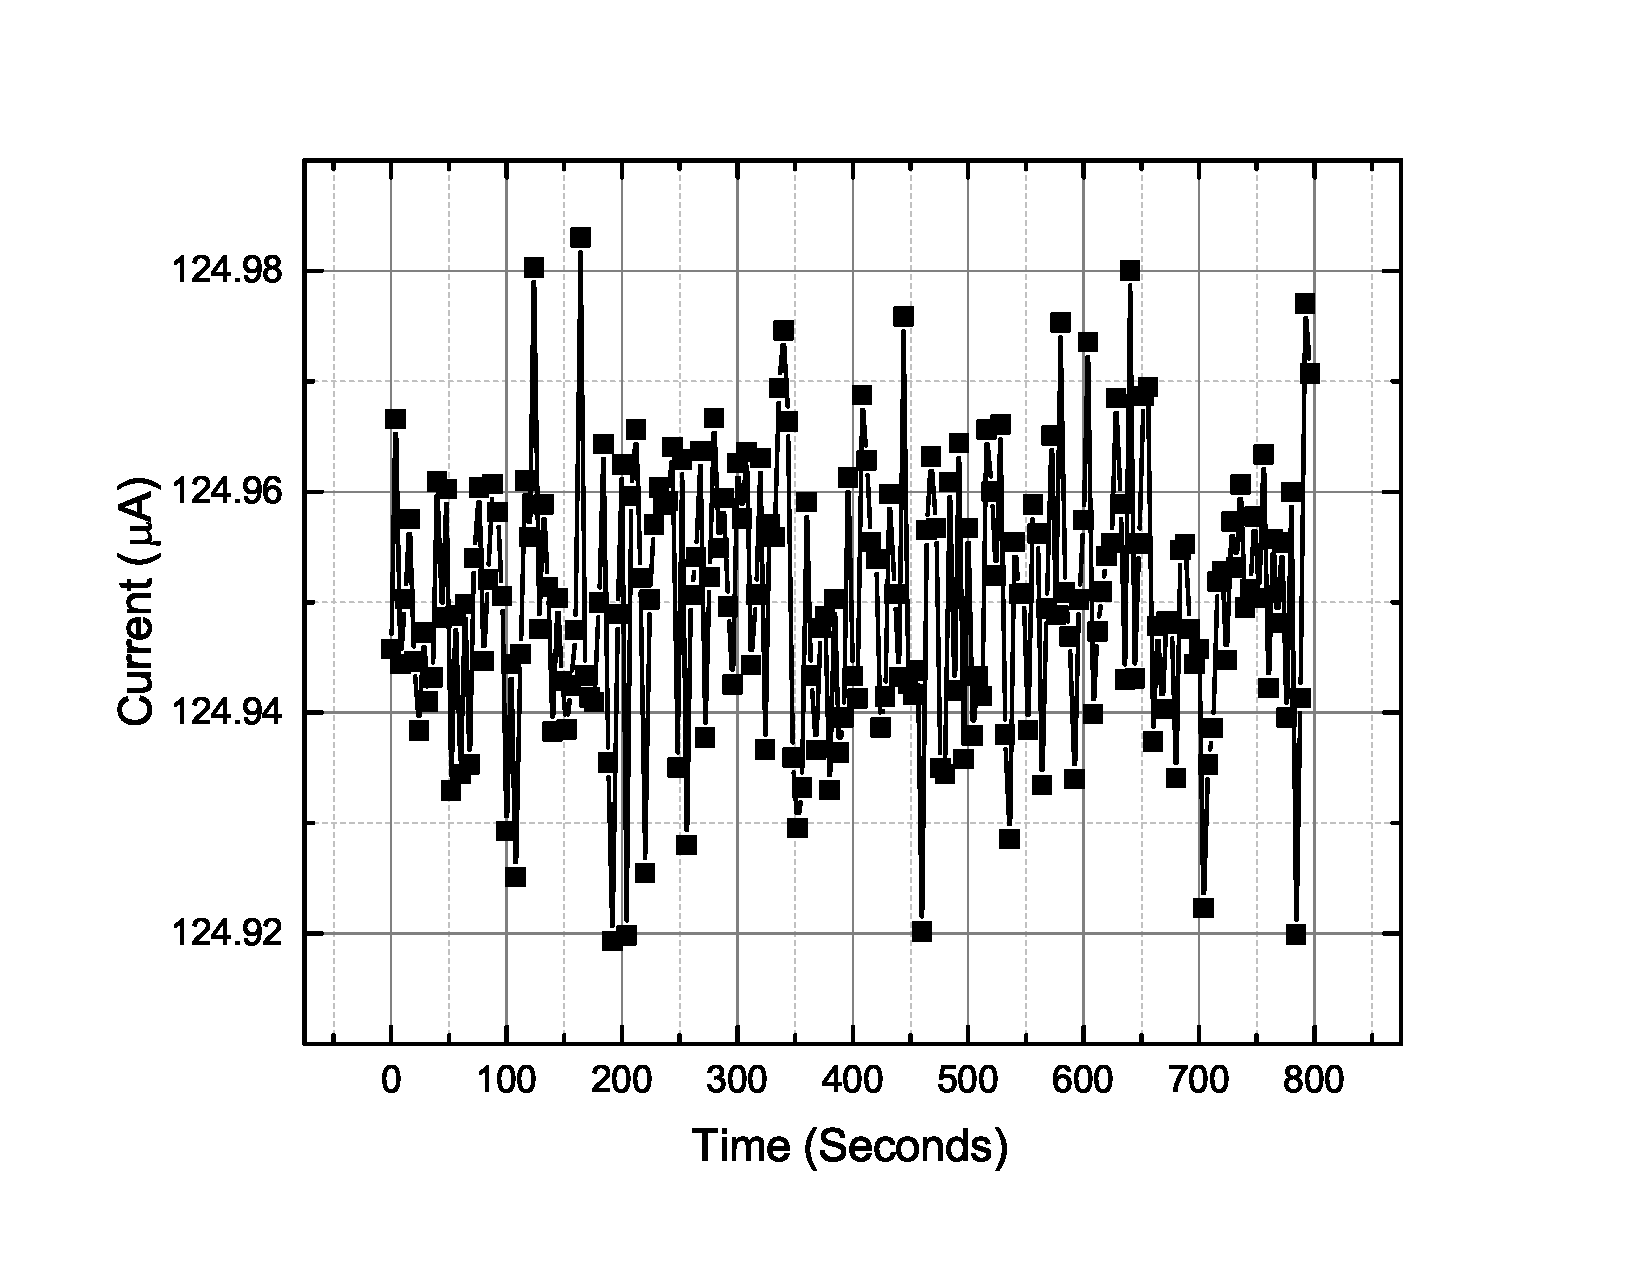
\includegraphics[width=0.35\paperwidth]{img/07/current_time.eps}
                    &
                    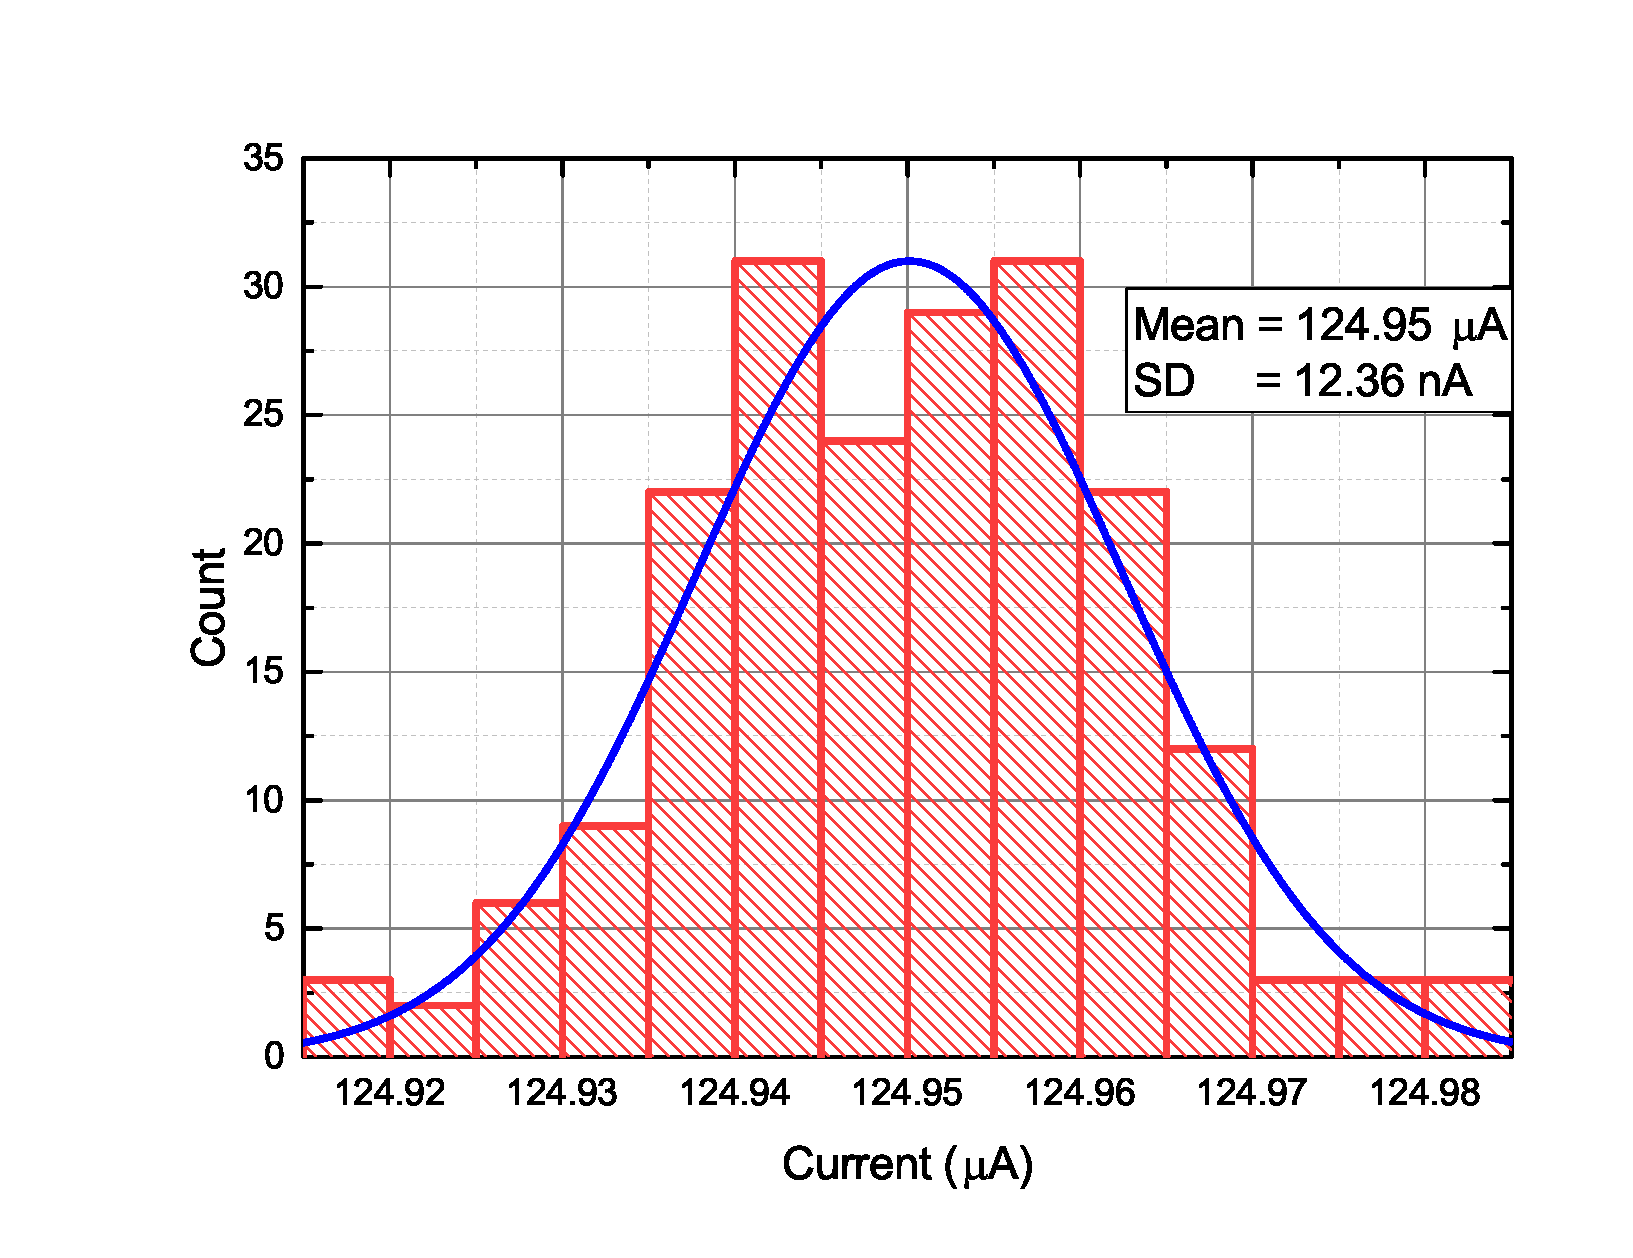
\includegraphics[width=0.35\paperwidth]{img/07/current_hist.eps}
                \end{tabular}
            \end{center}
            \caption{Current noise in time and histogram}
            \label{Current_Stability}
        \end{table}

    \subsection{Load range}
        Output load was changed in identical manner as in simulation, to tests its fidelity. Simulation and build model shown same range and stability - confirming the design. Current source works as intended for loads between \SI{1.4}{\kilo\ohm} and \SI{22.5}{\kilo\ohm} (figure \ref{Current_sensor_output_characteristics}).
        \begin{figure}[H]
            \centering
            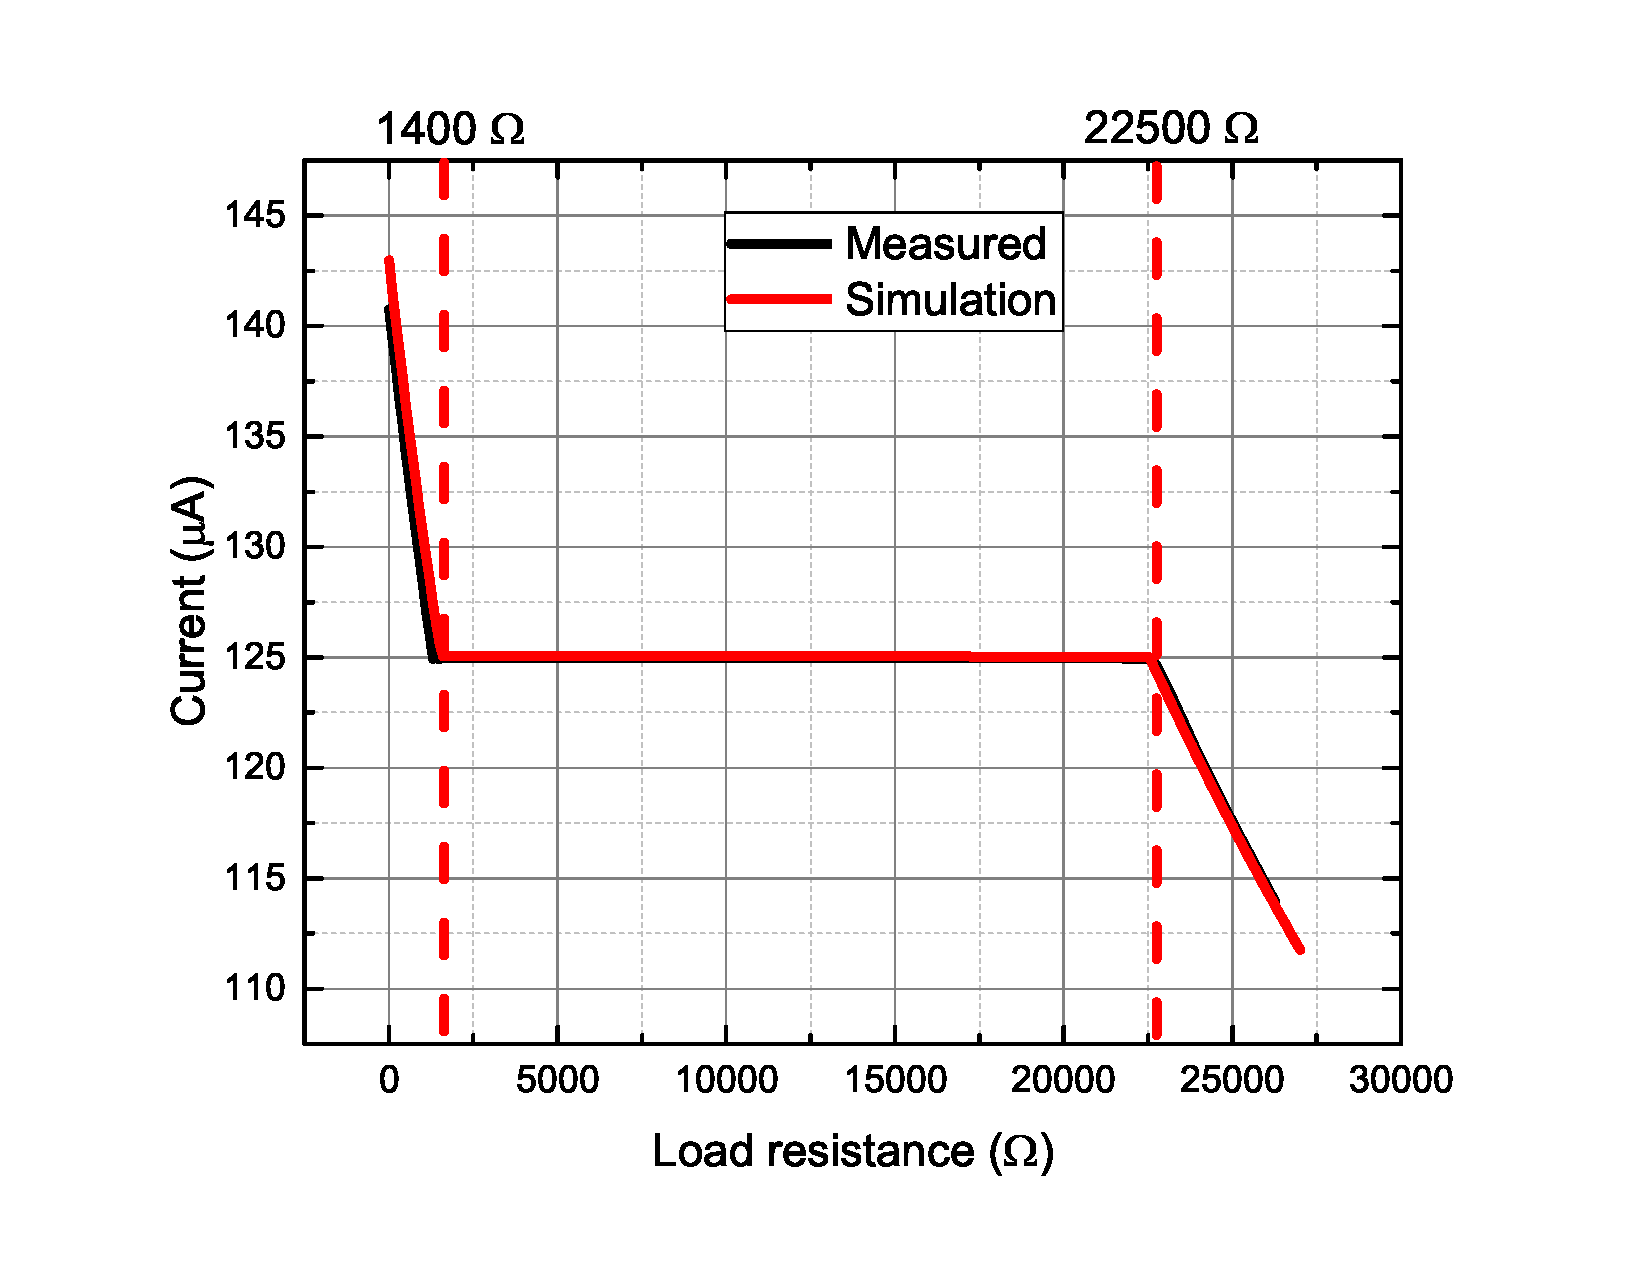
\includegraphics[width=0.6\paperwidth]{img/07/output_resistance.eps}
            \caption{Current sensor output characteristics}
            \label{Current_sensor_output_characteristics}
        \end{figure}

    \subsection{Temperature stability}
        Temperature was swept from $20$ to \SI{70}{\degreeCelsius}, no detectable changes were measured by available meter, therefore it is assumed that current source changes lower than about \SI{20}{\nano\ampere} in this temperature range.

\section{MOS settling}
    After enabling measurement channel for threshold voltage it takes a lot of time to fully stabilize its value. Instead of pre-enabling, same time method was used. ADC takes measurement of threshold voltage at precisely specified time after enabling power. On figure \ref{MOS_settling} 10 runs of measured voltage vs time are plotted, proving this method is stable within \SI{20}{\uV}.

    \begin{figure}[H]
        \centering
        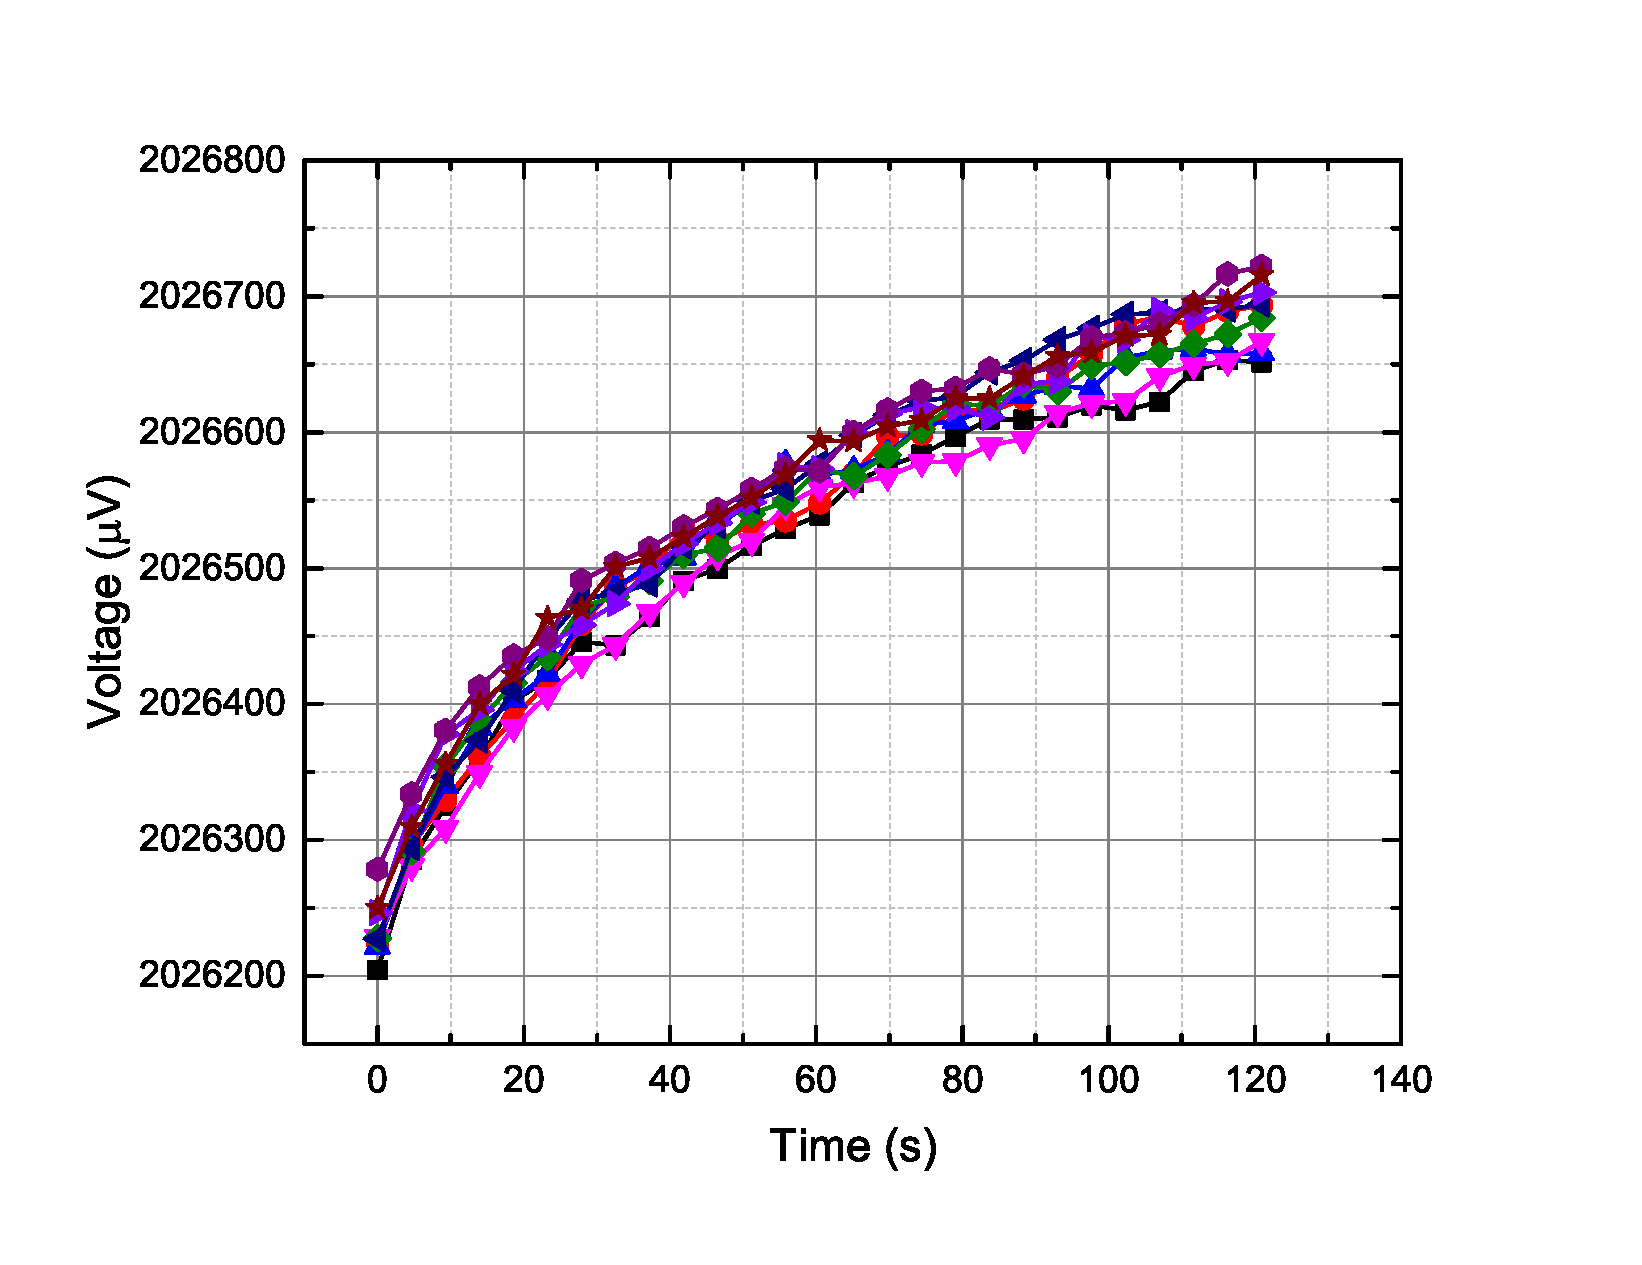
\includegraphics[width=0.8\paperwidth]{img/07/MOS_settling.eps}
        \caption{10 runs of MOS voltage setting}
        \label{MOS_settling}
    \end{figure}

\section{Measurement noise}
    Most important noise figure is system noise - ADC reading noise floor during nominal work.

    Because even smallest temperature changes cause ADC reading to shift (due to threshold/diode voltage shift) this efect had to be eliminated to measure noise. For this purpose DC notch filter was used in post-processing, to eliminate any DC bias during measurement. Transfer function of this filter is shown on figure TODO. Example of filtration is shown on figure TODO.

    Image: [przed filtracją] -> po filtracji

    Image: ch-ka filtru

    \subsection{Diode}
        Image: time + histogram

        Noise on temperature measurement channel have standard deviation of $1.2 uV$
    \subsection{Threshold voltage}
        Image: time + histogram

        Noise on threshold voltage measurement channel have standard deviation of $8.2 uV$

    \subsection{Interpretation}
        Because the only difference between temperature and threshold voltage channels is semiconductor itself, source of noise can be estimated from significant difference between them.

        Estimated current source noise is $2 nA$.
        This value can be confirmed by calculations, reference voltage LT1634 have low-frequency noise of $U_N = \SI{15}{\uV}$, this value is directly across series resistor, therefore $I_{NOISE} = U_N/R = \SI{1.5}{\nA}$. Noise output from LTSpice:



\section{Temperature characteristics}
    By sweeping temperature from \SI{0}{\degreeCelsius} up to \SI{75}{\degreeCelsius} temperature dependency charts were obtained for the device.

    \subsection{Diode}
        Diode response (ref) is alsost ideally linear.

        Image: chart + dopasowanie

    \subsection{Threshold voltage}
        Threshold voltage (ref) tends to be non-linear, but quadratic equation can be fitted to it.

        Image: chart + dopasowanie


\section{Temperature compensation stability}
    The sensor should be compensated for temperature, with assumption that temperature characteristic curves will not change during irradiation.

    During temperature sweep data was gathered, and post-processed applying thermal compensation (given by charts ref and ref). In full sensing range, sensor output shifts of maximum $\SI{400}{\uV}$, which reflects to TID measurement accuracy of \SI{\pm 1}{\rad}.



    

% Sensor tests
% - Digital
% -- Interface tests
% -- Software tests
% - Analog
% -- Measurement noise
% -- Temperature stability
% -- Ageing stability
% -- Irradiation tests

\chapter{Future work}

This chapter briefly describes required steps for the sensor to be able to fly on-board PW-Sat2.

\section{Qualification model}
    Firstly, the sensor will be implemented on PC-104 factor board, with all final components and procedures. This model is during designing (ref).

    Image: PC104-ze złączami

    On this model all software tests (on flat-sat) will be done, as well as final confirmation of design (thermal, radiation and time-stability tests). This board will qualify sensor design and software for flight use.

\section{Flight model}
    At the end final flight version of the PCB will be manufactured. In the principle, it should be identical to Qualification Model, but handling procedures will be much more strict. Additionally, on flight model only thermal calibration will be made, without further stress-testing. During integration, final version of the sensor on PC104-board will be placed on electronics stack inside PW-Sat2.

% Future work
% - Proto-flight model
% - Flight model

\chapter{Summary}
    The engineering model of the sensor was designed and preliminarily tested. This is a solid foundation to further work, which will result in the flight-ready version of the sensor. This model allowed for testing of the concept and possible solutions of sensor components, proving the design.

    Tests have proven the fidelity of measurements - assumed resolution and range are beyond the requirements. Designed sensor parameters are shown in table \ref{sensor_results_parameters}.

    \begin{table}[H]
        \caption{Finished sensor parameters}
        \label{sensor_results_parameters}
        \begin{center}
            \begin{tabular}{r|l}
                \textbf{Parameter} & \textbf{Result} \\ \hline
                Sensor resolution & \SI{0.003}{\rad}, \\
                Sensor accuracy & \SI{1}{\rad}, \\
                Sensor range & \SI{10}{\kilo\rad}, \\
                Operating temperature range & \SI{0}{\degreeCelsius} to \SI{70}{\degreeCelsius}, \\
                Communication protocol & $I^2C$, \\
                Sensor supply voltage & \SI{5}{\volt}, \\
                Sensor power consumption & \SI{0.125}{\watt}, \\
                Radiation tolerance & $>~\SI{15}{\kilo\rad}$ \\

            \end{tabular}
        \end{center}
    \end{table}

    This thesis resulted in a fully integrated, ready to use sensor which can be used as a preliminary calibration check model. It was designed for a space environment, with the limitations and requirements of CubeSat satellite in mind. During testing, the sensor design was proved through the conduction of tests. Moreover, since its size and requirements on the bus have been limited, broader possibilities of manufacturing this sensor as a separate module exist for other CubeSat missions.

    As a next step, this model has to be tested more throughly - especially radiation tests and calibration. Later, qualification and flight models will be manufactured, hopefully leading to sensor launch on PW-Sat2 satellite at the end of year 2017, where it can be tested in target space conditions.

% Summary
%
% Figures
% Tables



\appendix
\printbibliography

\end{document}
